\section{Determining hardware delay} \label{sec:HardwareDelay}

The following section describes testing of the conversion delay in the chosen implementation platform.

\subsection{Purpose}

The conversion delay inside the platform is in this project not neglectable and has to be measured and accounted for. With the conversion delay determined it is possible to simulate more accurate. % It is necessary to account for the delay if implentation should ocour.


\subsection{Settings/Description}

To measure the delay of the conversion time the codec is setup to the desired sampling frequency. This is done 





\subsection{Choice of equipment}


\subsection{AAU num list}

\begin{table}[H]
	\centering
	\ra{1.3}
	\begin{tabular}{ c c c } \toprule
		{Item}	& {Description} 						& {AAU-no}. \\ \bottomrule 
		1	&	Spectrum Digital TMS320C5515 eZdsp	& NaN	\\
		2	&	Digilent Analog Discovery 2	& NaN		\\
		3	&	DSP Freedom Board Rev. 1 & NaN		\\
		4	&	Computer w. Waveform 2015					& NaN		\\
		\bottomrule
	\end{tabular}
	\caption{Table over equipment used in test.}
	\label{tab:MeasDelayTable}
\end{table}

\subsection{Diagram}

\begin{figure}[H]
	\centering
	\tikzsetnextfilename{DelaySetupExperiment}
	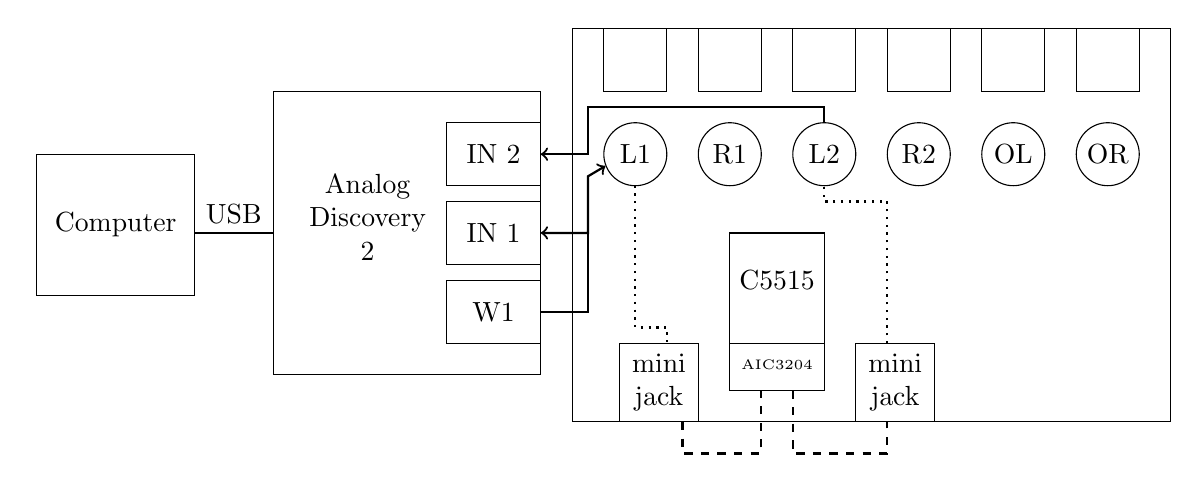
\begin{tikzpicture}
\draw  (3.8,3.4) rectangle (-3.8,-1.6);
\draw  (-1.8,0.8) rectangle (-0.6,-1.2);


\draw  (-1.8,1.8) node (3) {R1} ellipse (0.4 and 0.4);
\draw  (-3,1.8) node (v3) {L1} ellipse (0.4 and 0.4);

\draw  (1.8,1.8) node (v3) {OL} ellipse (0.4 and 0.4);
\draw  (3,1.8) node (v3) {OR} ellipse (0.4 and 0.4);

\draw  (-0.6,1.8) node (v5) {L2} ellipse (0.4 and 0.4);
\draw  (0.6,1.8) node (v3) {R2} ellipse (0.4 and 0.4);

\draw  (-2.2,-1.6) rectangle node [text width = 1cm, align=center] {mini jack} (-3.2,-0.6);

\draw  (0.8,-1.6) rectangle node [text width = 1cm,align=center] {mini jack} (-0.2,-0.6);


\draw  (-3.4,3.4) rectangle (-2.6,2.6);
\draw  (-2.2,2.6) rectangle (-1.4,3.4);
\draw  (-1,2.6) rectangle (-0.2,3.4);
\draw  (0.2,2.6) rectangle (1,3.4);
\draw  (1.4,2.6) rectangle (2.2,3.4);
\draw  (2.6,2.6) rectangle (3.4,3.4);


\draw [dotted,thick](0.2,-0.6) -- (0.2,1.2) -- (-0.6,1.2) -- (-0.6,1.4);
\draw [dotted,thick](-3,1.4) -- (-3,-0.4) -- (-2.6,-0.4) -- (-2.6,-0.6);

\draw [thick,dashed](-2.4,-1.6) -- (-2.4,-2) -- (-1.4,-2) -- (-1.4,-1.2);
\draw [thick,dashed](-1,-1.2) -- (-1,-2) -- (0.2,-2) -- (0.2,-1.6);
\node at (-1.2,0.2) {C5515};
\node [] at (-1.2,-0.88) {\tiny{AIC3204}};
\draw (-0.6,-0.6) -- (-1.8,-0.6);

\draw  (-4.2,-1) rectangle (-7.6,2.6);
\draw  (-8.6,0) rectangle node [text width = 2cm,align=center] {Computer} (-10.6,1.8);

\draw  (-4.2,2.2) rectangle node [text width = 1cm,align=center] {IN 2} (-5.4,1.4);
\draw  (-4.2,1.2) rectangle node [text width = 1cm,align=center] {IN 1} (-5.4,0.4);
\draw  (-4.2,0.2) rectangle node [text width = 1cm,align=center] {W1} (-5.4,-0.6);
\draw (v3);
\draw [thick,->](-0.6,2.2) -- (-0.6,2.4) -- (-3.6,2.4) -- (-3.6,1.8) -- (-4.2,1.8);

\node [text width = 1.75cm,align=center] at (-6.4,1) {Analog Discovery \\ 2};


\draw (-8.6,0.8) -- node [above] {USB} (-7.6,0.8);
\draw[thick,<->] (-4.2,0.8) -- (-3.6,0.8) node (v1) {} -- (-3.6,1.52) -- (-3.38,1.65);

\draw[thick] (-4.2,-0.2) -- (-3.6,-0.2) -- (-3.6,0.8);
\end{tikzpicture}
	\caption{Schematic overview of the experiment.}
	\label{fig:SchematicDelayExperiment}
\end{figure}

\subsection{Picture}

\begin{figure}[H]
	\centering
\includegraphics[width=0.75\textwidth]{Hardware/DelaySetup}
	\caption{Schematic overview of the experiment.}
	\label{fig:DelayExperimentSetu}
\end{figure}


\subsection{Control and calibration}

\subsection{Equipment settings}



\subsection{Procedure}

\begin{lstlisting} [language=C]
void main( void )
{
/* Initialize Board and Codec - look in "aic3204_setup.h" */
USBSTK5515_init();
codec_init ();
initAll();

while ( 1 )
{
/* Read Digital audio */
while((Rcv & I2S0_IR) == 0);  // Wait for interrupt pending flag
	data3 = I2S0_W0_MSW_R;  // 16 bit left channel received audio data
	data1 = I2S0_W0_LSW_R;
	data4 = I2S0_W1_MSW_R;  // 16 bit right channel received audio data
	data2 = I2S0_W1_LSW_R;


//asm(" bset XF");


/* Write Digital audio */
	while((Xmit & I2S0_IR) == 0);  // Wait for interrupt pending flag
	asm(" bset XF");
	I2S0_W0_MSW_W = data3;  // 16 bit left channel transmit audio data
	I2S0_W0_LSW_W = 0;
	I2S0_W1_MSW_W = data4;  // 16 bit right channel transmit audio data
	I2S0_W1_LSW_W = 0;
	}
}
\end{lstlisting}



\subsection{Data Extraction}

\subsection{Analysis}

\begin{figure}[H]
	\centering
	\tikzsetnextfilename{DelaySetupCSVRead}
	% This file was created by matlab2tikz.
%
%The latest updates can be retrieved from
%  http://www.mathworks.com/matlabcentral/fileexchange/22022-matlab2tikz-matlab2tikz
%where you can also make suggestions and rate matlab2tikz.
%
\definecolor{mycolor1}{rgb}{0.00000,0.44700,0.74100}%
\definecolor{mycolor2}{rgb}{0.85000,0.32500,0.09800}%
\definecolor{mycolor3}{rgb}{0.92900,0.69400,0.12500}%
\definecolor{mycolor4}{rgb}{0.49400,0.18400,0.55600}%
%
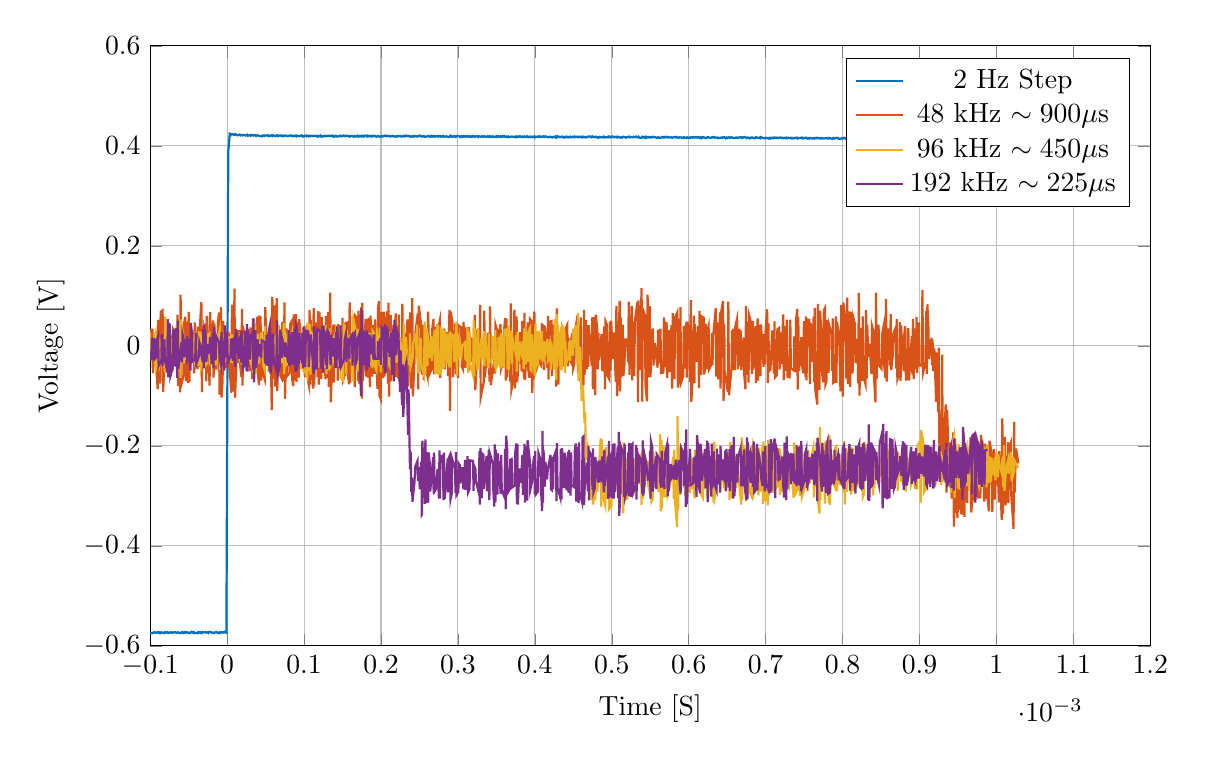
\begin{tikzpicture}

\begin{axis}[%
width=5in,
height=3in,
xmajorgrids,
xminorgrids,
ymajorgrids,
yminorgrids,
scale only axis,
xmin=-0.0001,
xmax=0.0012,
ymin=-0.6,
ymax=0.6,
ylabel={Voltage [V]},
xlabel={Time [S]},
axis background/.style={fill=white},
%legend style={legend cell align=left,align=left,draw=white!15!black}
]
\addplot [color=mycolor1,solid,thick]
  table[row sep=crcr]{%
-0.00010012	-0.5733\\
-0.00010012	-0.5733\\
-9.9069e-05	-0.5743\\
-9.6969e-05	-0.57464\\
-9.4869e-05	-0.57296\\
-9.4269e-05	-0.57263\\
-9.2169e-05	-0.5743\\
-9.2169e-05	-0.5743\\
-9.0519e-05	-0.57296\\
-8.8719e-05	-0.57296\\
-8.8119e-05	-0.57464\\
-8.6619e-05	-0.57464\\
-8.5719e-05	-0.57296\\
-8.4369e-05	-0.5733\\
-8.1969e-05	-0.57464\\
-8.1669e-05	-0.5743\\
-8.0619e-05	-0.57263\\
-7.8369e-05	-0.57363\\
-7.7619e-05	-0.57263\\
-7.5669e-05	-0.5743\\
-7.4169e-05	-0.57296\\
-7.3419e-05	-0.57263\\
-7.1619e-05	-0.57397\\
-7.1469e-05	-0.57397\\
-7.0719e-05	-0.57296\\
-6.8769e-05	-0.5733\\
-6.7569e-05	-0.57263\\
-6.5619e-05	-0.57397\\
-6.3969e-05	-0.57296\\
-6.3669e-05	-0.57296\\
-6.1119e-05	-0.57464\\
-6.0969e-05	-0.57464\\
-5.8869e-05	-0.57263\\
-5.7819e-05	-0.57296\\
-5.7369e-05	-0.5743\\
-5.5569e-05	-0.57263\\
-5.4519e-05	-0.57397\\
-5.3019e-05	-0.57263\\
-5.1969e-05	-0.57363\\
-5.0469e-05	-0.5733\\
-4.9419e-05	-0.57464\\
-4.8069e-05	-0.57397\\
-4.6419e-05	-0.57195\\
-4.5069e-05	-0.57229\\
-4.3719e-05	-0.5743\\
-4.2819e-05	-0.57296\\
-4.1919e-05	-0.57397\\
-3.8619e-05	-0.57464\\
-3.8019e-05	-0.5733\\
-3.7569e-05	-0.5743\\
-3.5769e-05	-0.57263\\
-3.4419e-05	-0.57296\\
-3.3819e-05	-0.5743\\
-3.2319e-05	-0.57263\\
-3.1869e-05	-0.57363\\
-2.8719e-05	-0.57229\\
-2.7369e-05	-0.57363\\
-2.7219e-05	-0.57363\\
-2.4819e-05	-0.57263\\
-2.4519e-05	-0.5733\\
-2.4369e-05	-0.57263\\
-2.1669e-05	-0.57229\\
-2.0919e-05	-0.57363\\
-1.8969e-05	-0.5733\\
-1.8369e-05	-0.5743\\
-1.6869e-05	-0.57397\\
-1.5219e-05	-0.57263\\
-1.3119e-05	-0.57263\\
-1.1919e-05	-0.5743\\
-9.8194e-06	-0.57464\\
-9.3694e-06	-0.5733\\
-8.7694e-06	-0.57397\\
-7.5694e-06	-0.57263\\
-6.2194e-06	-0.57263\\
-5.1694e-06	-0.57363\\
-3.2194e-06	-0.57195\\
-2.1694e-06	-0.57363\\
-9.6936e-07	-0.57397\\
1.4306e-06	0.38857\\
1.4306e-06	0.38857\\
3.3806e-06	0.4238\\
4.7306e-06	0.42212\\
5.0306e-06	0.42346\\
7.1306e-06	0.42313\\
8.7806e-06	0.42178\\
9.5306e-06	0.42178\\
1.0431e-05	0.42346\\
1.1781e-05	0.42212\\
1.2831e-05	0.42111\\
1.4331e-05	0.42111\\
1.5981e-05	0.42245\\
1.7331e-05	0.42111\\
1.7631e-05	0.42178\\
1.9731e-05	0.42078\\
2.0631e-05	0.42178\\
2.2131e-05	0.42145\\
2.3931e-05	0.42044\\
2.6031e-05	0.42212\\
2.6781e-05	0.42011\\
2.7981e-05	0.42044\\
2.9631e-05	0.42145\\
3.0081e-05	0.42145\\
3.0831e-05	0.42011\\
3.3081e-05	0.42178\\
3.4731e-05	0.42044\\
3.6231e-05	0.42145\\
3.7581e-05	0.41977\\
3.7731e-05	0.42011\\
3.9231e-05	0.42111\\
4.0431e-05	0.42078\\
4.1631e-05	0.41943\\
4.3581e-05	0.41977\\
4.4931e-05	0.41876\\
4.5531e-05	0.4191\\
4.6581e-05	0.42078\\
4.8231e-05	0.41977\\
4.8531e-05	0.42044\\
5.2281e-05	0.42078\\
5.3181e-05	0.41977\\
5.3481e-05	0.42044\\
5.3931e-05	0.41943\\
5.6181e-05	0.41977\\
5.7531e-05	0.42111\\
5.8731e-05	0.41977\\
5.9181e-05	0.42111\\
6.1131e-05	0.42044\\
6.2031e-05	0.41943\\
6.3831e-05	0.41943\\
6.4731e-05	0.42111\\
6.6681e-05	0.41943\\
6.7581e-05	0.42044\\
6.9831e-05	0.42078\\
7.0731e-05	0.41943\\
7.1781e-05	0.42044\\
7.3431e-05	0.4191\\
7.4481e-05	0.41943\\
7.4631e-05	0.42044\\
7.6731e-05	0.42044\\
7.8531e-05	0.4191\\
7.9431e-05	0.41943\\
8.1531e-05	0.42078\\
8.2281e-05	0.42078\\
8.4231e-05	0.41943\\
8.4531e-05	0.42011\\
8.5431e-05	0.4191\\
8.8881e-05	0.42044\\
8.9631e-05	0.4191\\
8.9781e-05	0.41943\\
9.0531e-05	0.42044\\
9.2481e-05	0.42011\\
9.3231e-05	0.4191\\
9.6081e-05	0.42044\\
9.7431e-05	0.41943\\
9.7581e-05	0.42011\\
9.8781e-05	0.41843\\
0.00010013	0.4191\\
0.00010118	0.42044\\
0.00010283	0.4191\\
0.00010358	0.42044\\
0.00010553	0.4191\\
0.00010598	0.42011\\
0.00010793	0.4191\\
0.00010838	0.42011\\
0.00011078	0.42011\\
0.00011183	0.4191\\
0.00011318	0.42011\\
0.00011573	0.4191\\
0.00011663	0.42011\\
0.00011798	0.41809\\
0.00011843	0.41843\\
0.00011948	0.41977\\
0.00012143	0.41876\\
0.00012188	0.42044\\
0.00012413	0.41843\\
0.00012623	0.42011\\
0.00012623	0.42011\\
0.00012803	0.4191\\
0.00012878	0.4191\\
0.00012908	0.42011\\
0.00013148	0.41943\\
0.00013253	0.42044\\
0.00013553	0.4191\\
0.00013643	0.42044\\
0.00013703	0.42044\\
0.00013853	0.41809\\
0.00013913	0.41876\\
0.00014093	0.42011\\
0.00014183	0.41977\\
0.00014213	0.41876\\
0.00014468	0.41876\\
0.00014663	0.41977\\
0.00014708	0.42011\\
0.00014753	0.4191\\
0.00014963	0.4191\\
0.00015113	0.42078\\
0.00015293	0.4191\\
0.00015473	0.42011\\
0.00015488	0.42044\\
0.00015698	0.4191\\
0.00015743	0.41977\\
0.00015953	0.41843\\
0.00015998	0.4191\\
0.00016148	0.41977\\
0.00016253	0.41977\\
0.00016448	0.41809\\
0.00016553	0.41977\\
0.00016763	0.41843\\
0.00016853	0.41843\\
0.00016943	0.42011\\
0.00017093	0.41843\\
0.00017153	0.41977\\
0.00017453	0.41843\\
0.00017528	0.42011\\
0.00017573	0.42044\\
0.00017768	0.41843\\
0.00017813	0.4191\\
0.00017888	0.42044\\
0.00018188	0.41876\\
0.00018233	0.42011\\
0.00018338	0.41876\\
0.00018473	0.42011\\
0.00018713	0.41843\\
0.00018818	0.41977\\
0.00018953	0.41876\\
0.00019058	0.42011\\
0.00019208	0.41977\\
0.00019388	0.41809\\
0.00019388	0.41809\\
0.00019598	0.41977\\
0.00019643	0.41977\\
0.00019868	0.41809\\
0.00019943	0.41843\\
0.00020048	0.41943\\
0.00020183	0.41876\\
0.00020198	0.41943\\
0.00020423	0.41943\\
0.00020498	0.42044\\
0.00020678	0.42011\\
0.00020708	0.4191\\
0.00021023	0.41977\\
0.00021203	0.41843\\
0.00021203	0.41843\\
0.00021383	0.41977\\
0.00021473	0.42011\\
0.00021593	0.41876\\
0.00021728	0.4191\\
0.00021923	0.41809\\
0.00021983	0.41843\\
0.00022088	0.41977\\
0.00022238	0.41876\\
0.00022358	0.41977\\
0.00022568	0.41977\\
0.00022613	0.41843\\
0.00022823	0.41843\\
0.00022958	0.42011\\
0.00023093	0.41876\\
0.00023258	0.42044\\
0.00023288	0.42044\\
0.00023468	0.4191\\
0.00023603	0.42011\\
0.00023738	0.41876\\
0.00023828	0.4191\\
0.00023903	0.41809\\
0.00024233	0.41977\\
0.00024293	0.41843\\
0.00024338	0.41876\\
0.00024473	0.41943\\
0.00024698	0.41843\\
0.00024803	0.41943\\
0.00024848	0.4191\\
0.00025058	0.42044\\
0.00025103	0.41943\\
0.00025298	0.41843\\
0.00025373	0.41876\\
0.00025418	0.41943\\
0.00025628	0.4191\\
0.00025643	0.41809\\
0.00025928	0.41843\\
0.00026138	0.41977\\
0.00026138	0.41977\\
0.00026333	0.41809\\
0.00026453	0.41843\\
0.00026513	0.42011\\
0.00026663	0.41977\\
0.00026708	0.41843\\
0.00026933	0.41977\\
0.00026978	0.41843\\
0.00027353	0.41943\\
0.00027443	0.41843\\
0.00027443	0.41843\\
0.00027518	0.41943\\
0.00027713	0.41843\\
0.00027728	0.41943\\
0.00027968	0.41843\\
0.00028088	0.41977\\
0.00028238	0.41809\\
0.00028478	0.4191\\
0.00028478	0.4191\\
0.00028673	0.41776\\
0.00028853	0.41776\\
0.00029003	0.42011\\
0.00029003	0.42011\\
0.00029078	0.41876\\
0.00029258	0.4191\\
0.00029288	0.41809\\
0.00029573	0.41943\\
0.00029708	0.41776\\
0.00029783	0.41843\\
0.00029858	0.41977\\
0.00030038	0.41977\\
0.00030278	0.41776\\
0.00030323	0.41742\\
0.00030458	0.41943\\
0.00030608	0.4191\\
0.00030623	0.41809\\
0.00030863	0.41943\\
0.00030938	0.41809\\
0.00031148	0.41943\\
0.00031283	0.41809\\
0.00031373	0.41943\\
0.00031553	0.41809\\
0.00031658	0.4191\\
0.00031793	0.41776\\
0.00031868	0.41843\\
0.00031973	0.41977\\
0.00032123	0.4191\\
0.00032153	0.41809\\
0.00032543	0.41943\\
0.00032633	0.41776\\
0.00032663	0.41843\\
0.00032783	0.4191\\
0.00032963	0.41809\\
0.00033128	0.4191\\
0.00033173	0.4191\\
0.00033263	0.41776\\
0.00033443	0.4191\\
0.00033653	0.41809\\
0.00033743	0.41776\\
0.00033863	0.4191\\
0.00033998	0.41776\\
0.00034133	0.4191\\
0.00034208	0.41876\\
0.00034253	0.41776\\
0.00034538	0.4191\\
0.00034643	0.41742\\
0.00034823	0.41776\\
0.00034988	0.4191\\
0.00035048	0.41809\\
0.00035108	0.41943\\
0.00035243	0.4191\\
0.00035363	0.41776\\
0.00035543	0.4191\\
0.00035618	0.41776\\
0.00035798	0.4191\\
0.00035828	0.41843\\
0.00036038	0.41943\\
0.00036128	0.41809\\
0.00036278	0.41876\\
0.00036458	0.41742\\
0.00036548	0.41843\\
0.00036578	0.41742\\
0.00036803	0.41776\\
0.00037028	0.41876\\
0.00037073	0.41843\\
0.00037283	0.41742\\
0.00037508	0.41876\\
0.00037583	0.41709\\
0.00037583	0.41709\\
0.00037808	0.41876\\
0.00037883	0.41776\\
0.00038063	0.4191\\
0.00038183	0.41843\\
0.00038258	0.41742\\
0.00038393	0.41843\\
0.00038513	0.41742\\
0.00038648	0.41876\\
0.00038873	0.41742\\
0.00038888	0.41742\\
0.00038993	0.4191\\
0.00039158	0.41742\\
0.00039368	0.41843\\
0.00039443	0.41742\\
0.00039578	0.41843\\
0.00039728	0.41742\\
0.00039923	0.41843\\
0.00039953	0.41776\\
0.00039968	0.41876\\
0.00040178	0.41776\\
0.00040448	0.41876\\
0.00040538	0.41776\\
0.00040688	0.4191\\
0.00040718	0.41876\\
0.00040793	0.41776\\
0.00041153	0.4191\\
0.00041213	0.41742\\
0.00041228	0.41742\\
0.00041288	0.41876\\
0.00041528	0.41843\\
0.00041588	0.41742\\
0.00041783	0.41709\\
0.00041978	0.41843\\
0.00042008	0.41809\\
0.00042218	0.41675\\
0.00042278	0.41675\\
0.00042398	0.41809\\
0.00042638	0.41675\\
0.00042698	0.41843\\
0.00042833	0.41642\\
0.00042938	0.4191\\
0.00043103	0.41843\\
0.00043268	0.41709\\
0.00043298	0.41709\\
0.00043508	0.41843\\
0.00043568	0.41843\\
0.00043748	0.41642\\
0.00043853	0.41675\\
0.00043928	0.41776\\
0.00044078	0.41709\\
0.00044123	0.41843\\
0.00044393	0.41675\\
0.00044573	0.41843\\
0.00044603	0.41843\\
0.00044693	0.41709\\
0.00044888	0.41742\\
0.00044948	0.41843\\
0.00045143	0.41709\\
0.00045203	0.41843\\
0.00045533	0.41809\\
0.00045623	0.41709\\
0.00045698	0.41709\\
0.00045713	0.41809\\
0.00045998	0.41809\\
0.00046133	0.41642\\
0.00046178	0.41642\\
0.00046253	0.41843\\
0.00046463	0.41776\\
0.00046583	0.41675\\
0.00046688	0.41709\\
0.00046898	0.41843\\
0.00046958	0.41776\\
0.00047063	0.41876\\
0.00047213	0.41876\\
0.00047348	0.41709\\
0.00047498	0.41876\\
0.00047573	0.41742\\
0.00047768	0.41809\\
0.00047933	0.41709\\
0.00048023	0.41809\\
0.00048248	0.41574\\
0.00048248	0.41574\\
0.00048413	0.41809\\
0.00048518	0.41776\\
0.00048623	0.41675\\
0.00048863	0.41809\\
0.00048983	0.41675\\
0.00049028	0.41809\\
0.00049118	0.41709\\
0.00049523	0.41709\\
0.00049538	0.41843\\
0.00049598	0.41876\\
0.00049763	0.41709\\
0.00049808	0.41776\\
0.00049853	0.41709\\
0.00050123	0.41876\\
0.00050213	0.41709\\
0.00050363	0.41709\\
0.00050498	0.41809\\
0.00050693	0.41675\\
0.00050708	0.41809\\
0.00050873	0.41809\\
0.00051113	0.41642\\
0.00051173	0.41608\\
0.00051308	0.41742\\
0.00051368	0.41675\\
0.00051488	0.41809\\
0.00051743	0.41742\\
0.00051833	0.41608\\
0.00051893	0.41675\\
0.00052028	0.41742\\
0.00052223	0.41843\\
0.00052328	0.41709\\
0.00052403	0.41809\\
0.00052643	0.41675\\
0.00052688	0.41709\\
0.00052823	0.41809\\
0.00052958	0.41742\\
0.00053168	0.41843\\
0.00053273	0.41709\\
0.00053453	0.41843\\
0.00053453	0.41843\\
0.00053528	0.41642\\
0.00053843	0.41608\\
0.00053948	0.41742\\
0.00053963	0.41675\\
0.00054158	0.41776\\
0.00054293	0.41608\\
0.00054428	0.41809\\
0.00054503	0.41608\\
0.00054698	0.41776\\
0.00054803	0.41776\\
0.00054878	0.41642\\
0.00055103	0.41776\\
0.00055193	0.41675\\
0.00055268	0.41675\\
0.00055403	0.41809\\
0.00055523	0.41776\\
0.00055688	0.41675\\
0.00055943	0.41574\\
0.00056048	0.41742\\
0.00056048	0.41742\\
0.00056243	0.41574\\
0.00056438	0.41642\\
0.00056573	0.41776\\
0.00056573	0.41776\\
0.00056783	0.41642\\
0.00056828	0.41675\\
0.00056858	0.41776\\
0.00057098	0.41675\\
0.00057158	0.41809\\
0.00057353	0.41742\\
0.00057443	0.41642\\
0.00057713	0.41709\\
0.00057833	0.41608\\
0.00057863	0.41642\\
0.00058118	0.41776\\
0.00058163	0.41742\\
0.00058358	0.41642\\
0.00058448	0.41776\\
0.00058598	0.41642\\
0.00058688	0.41574\\
0.00058823	0.41709\\
0.00059033	0.41675\\
0.00059138	0.41574\\
0.00059213	0.41574\\
0.00059378	0.41742\\
0.00059423	0.41709\\
0.00059483	0.41574\\
0.00059693	0.41574\\
0.00059783	0.41709\\
0.00059948	0.41574\\
0.00060143	0.41675\\
0.00060203	0.41608\\
0.00060368	0.41742\\
0.00060488	0.41642\\
0.00060563	0.41742\\
0.00060728	0.41642\\
0.00060893	0.41742\\
0.00061043	0.41709\\
0.00061133	0.41608\\
0.00061283	0.41742\\
0.00061478	0.41574\\
0.00061583	0.41709\\
0.00061658	0.41507\\
0.00061763	0.41574\\
0.00061853	0.41742\\
0.00062033	0.41675\\
0.00062123	0.41541\\
0.00062333	0.41574\\
0.00062423	0.41742\\
0.00062573	0.41709\\
0.00062813	0.41574\\
0.00062813	0.41574\\
0.00063053	0.41709\\
0.00063083	0.41675\\
0.00063173	0.41776\\
0.00063323	0.41742\\
0.00063383	0.41608\\
0.00063683	0.41675\\
0.00063788	0.41541\\
0.00063848	0.41608\\
0.00063923	0.41541\\
0.00064178	0.41541\\
0.00064223	0.41642\\
0.00064373	0.41574\\
0.00064448	0.41709\\
0.00064643	0.41709\\
0.00064778	0.41507\\
0.00064898	0.41675\\
0.00064988	0.41541\\
0.00065243	0.41742\\
0.00065348	0.41574\\
0.00065408	0.41608\\
0.00065543	0.41709\\
0.00065663	0.41675\\
0.00065738	0.41574\\
0.00066008	0.41541\\
0.00066173	0.41675\\
0.00066248	0.41642\\
0.00066353	0.41541\\
0.00066458	0.41541\\
0.00066473	0.41675\\
0.00066863	0.41709\\
0.00066938	0.41541\\
0.00066998	0.41574\\
0.00067178	0.41742\\
0.00067253	0.41776\\
0.00067478	0.41608\\
0.00067523	0.41541\\
0.00067658	0.41675\\
0.00067748	0.41642\\
0.00067958	0.41474\\
0.00068003	0.41541\\
0.00068093	0.41642\\
0.00068333	0.41642\\
0.00068438	0.41507\\
0.00068648	0.41507\\
0.00068723	0.41709\\
0.00068798	0.41709\\
0.00069023	0.41541\\
0.00069128	0.41541\\
0.00069293	0.41709\\
0.00069323	0.41608\\
0.00069368	0.41709\\
0.00069563	0.41642\\
0.00069698	0.41507\\
0.00069953	0.41507\\
0.00070088	0.41608\\
0.00070088	0.41608\\
0.00070328	0.41507\\
0.00070418	0.4144\\
0.00070553	0.41608\\
0.00070643	0.41474\\
0.00070793	0.41608\\
0.00070928	0.41608\\
0.00070958	0.41507\\
0.00071183	0.41541\\
0.00071198	0.41642\\
0.00071453	0.41541\\
0.00071498	0.41642\\
0.00071678	0.41541\\
0.00071858	0.41675\\
0.00071903	0.41675\\
0.00072068	0.41541\\
0.00072173	0.41608\\
0.00072308	0.41507\\
0.00072443	0.41608\\
0.00072638	0.41507\\
0.00072728	0.41642\\
0.00072848	0.41541\\
0.00072983	0.41608\\
0.00073028	0.41541\\
0.00073313	0.41608\\
0.00073418	0.41474\\
0.00073463	0.41541\\
0.00073523	0.41474\\
0.00073778	0.41574\\
0.00073808	0.41507\\
0.00074063	0.41642\\
0.00074168	0.4144\\
0.00074258	0.41507\\
0.00074273	0.41574\\
0.00074633	0.41608\\
0.00074663	0.41507\\
0.00074813	0.41474\\
0.00074858	0.41608\\
0.00075038	0.41507\\
0.00075263	0.41642\\
0.00075308	0.41574\\
0.00075413	0.4144\\
0.00075698	0.41574\\
0.00075713	0.41474\\
0.00075818	0.41541\\
0.00076028	0.4144\\
0.00076088	0.41474\\
0.00076178	0.41574\\
0.00076358	0.4144\\
0.00076448	0.41574\\
0.00076628	0.41507\\
0.00076658	0.41608\\
0.00076853	0.41574\\
0.00076988	0.41474\\
0.00077138	0.4144\\
0.00077183	0.41574\\
0.00077378	0.41541\\
0.00077453	0.4144\\
0.00077648	0.41474\\
0.00077858	0.41574\\
0.00077888	0.41541\\
0.00078023	0.4144\\
0.00078188	0.41474\\
0.00078203	0.41574\\
0.00078428	0.41507\\
0.00078623	0.41373\\
0.00078698	0.4144\\
0.00078803	0.41574\\
0.00078938	0.4144\\
0.00079148	0.41574\\
0.00079208	0.41608\\
0.00079403	0.41474\\
0.00079448	0.41507\\
0.00079508	0.41407\\
0.00079763	0.41373\\
0.00079853	0.41507\\
0.00079988	0.4144\\
0.00080198	0.41608\\
0.00080258	0.41574\\
0.00080378	0.41407\\
0.00080498	0.41541\\
0.00080738	0.4144\\
0.00080783	0.4144\\
0.00080813	0.41541\\
0.00081008	0.41507\\
0.00081128	0.41407\\
0.00081293	0.41507\\
0.00081398	0.4134\\
0.00081548	0.41507\\
0.00081683	0.41373\\
0.00081863	0.41373\\
0.00082013	0.41507\\
0.00082148	0.41407\\
0.00082223	0.41541\\
0.00082403	0.4134\\
0.00082538	0.41474\\
0.00082598	0.41407\\
0.00082658	0.41507\\
0.00082913	0.41407\\
0.00083048	0.41574\\
0.00083093	0.41474\\
0.00083198	0.41574\\
0.00083363	0.41474\\
0.00083438	0.41541\\
0.00083678	0.41608\\
0.00083798	0.41474\\
0.00083888	0.41541\\
0.00083963	0.41407\\
0.00084263	0.41541\\
0.00084293	0.41407\\
0.00084473	0.41373\\
0.00084638	0.41507\\
0.00084728	0.41407\\
0.00084743	0.41507\\
0.00084938	0.41574\\
0.00085103	0.41407\\
0.00085178	0.41407\\
0.00085238	0.41507\\
0.00085463	0.41474\\
0.00085658	0.41306\\
0.00085733	0.41306\\
0.00085823	0.41407\\
0.00085988	0.41373\\
0.00086168	0.41541\\
0.00086333	0.41541\\
0.00086423	0.41407\\
0.00086513	0.41407\\
0.00086603	0.41574\\
0.00086768	0.41373\\
0.00086978	0.41474\\
0.00086993	0.41373\\
0.00087128	0.41541\\
0.00087263	0.41474\\
0.00087293	0.41373\\
0.00087578	0.4144\\
0.00087728	0.4134\\
0.00087833	0.41306\\
0.00087893	0.4144\\
0.00088058	0.41373\\
0.00088283	0.41507\\
0.00088388	0.41474\\
0.00088523	0.41373\\
0.00088553	0.41407\\
0.00088778	0.41541\\
0.00088823	0.41574\\
0.00088988	0.41373\\
0.00089108	0.41507\\
0.00089333	0.41407\\
0.00089363	0.41474\\
0.00089558	0.41306\\
0.00089588	0.41373\\
0.00089648	0.41507\\
0.00089903	0.41474\\
0.00090053	0.4134\\
0.00090113	0.41474\\
0.00090128	0.41407\\
0.00090368	0.4144\\
0.00090473	0.41272\\
0.00090668	0.41373\\
0.00090788	0.41507\\
0.00090968	0.41306\\
0.00091118	0.41541\\
0.00091163	0.41541\\
0.00091403	0.41306\\
0.00091463	0.4144\\
0.00091553	0.41306\\
0.00091748	0.41373\\
0.00091763	0.4144\\
0.00092003	0.41474\\
0.00092048	0.4134\\
0.00092213	0.4144\\
0.00092258	0.4134\\
0.00092453	0.4134\\
0.00092618	0.41507\\
0.00092708	0.4144\\
0.00092888	0.4134\\
0.00093038	0.4134\\
0.00093098	0.41474\\
0.00093248	0.41407\\
0.00093443	0.41239\\
0.00093638	0.41239\\
0.00093758	0.4144\\
0.00093758	0.4144\\
0.00093848	0.41272\\
0.00094058	0.41306\\
0.00094178	0.4144\\
0.00094268	0.41306\\
0.00094283	0.4144\\
0.00094538	0.4144\\
0.00094598	0.41373\\
0.00094808	0.4134\\
0.00094898	0.41474\\
0.00095213	0.41474\\
0.00095258	0.41306\\
0.00095318	0.41373\\
0.00095408	0.41272\\
0.00095678	0.41272\\
0.00095813	0.41407\\
0.00095888	0.41507\\
0.00096053	0.41239\\
0.00096098	0.41306\\
0.00096248	0.41407\\
0.00096398	0.41407\\
0.00096473	0.41306\\
0.00096608	0.4134\\
0.00096743	0.41507\\
0.00096953	0.41507\\
0.00097058	0.4134\\
0.00097148	0.4144\\
0.00097283	0.41306\\
0.00097493	0.4134\\
0.00097658	0.41474\\
0.00097688	0.41474\\
0.00097868	0.41272\\
0.00097958	0.41239\\
0.00098093	0.41373\\
0.00098183	0.41407\\
0.00098348	0.41306\\
0.00098558	0.41306\\
0.00098648	0.4144\\
0.00098723	0.4134\\
0.00098828	0.4144\\
0.00098993	0.41306\\
0.00099173	0.41474\\
0.00099218	0.4144\\
0.00099368	0.41272\\
0.00099473	0.41306\\
0.00099713	0.4144\\
0.00099833	0.41407\\
0.00099953	0.41239\\
0.0010003	0.41239\\
0.0010013	0.41373\\
0.0010028	0.4144\\
0.0010045	0.41239\\
0.0010051	0.41272\\
0.0010061	0.41407\\
0.0010081	0.41407\\
0.0010099	0.41205\\
0.0010105	0.4134\\
0.0010115	0.41272\\
0.0010132	0.41239\\
0.0010142	0.41373\\
0.0010162	0.41306\\
0.0010181	0.4144\\
0.0010181	0.4144\\
0.0010184	0.41306\\
0.0010208	0.41407\\
0.0010226	0.41205\\
0.0010252	0.41239\\
0.0010259	0.41407\\
0.0010285	0.4134\\
};
\addlegendentry{2 Hz Step};

\addplot [color=mycolor2,solid,thick]
  table[row sep=crcr]{%
-0.00010012	-0.0041845\\
-9.9819e-05	0.033263\\
-9.7869e-05	-0.027255\\
-9.7119e-05	0.034266\\
-9.6519e-05	-0.054672\\
-9.3219e-05	0.0055117\\
-9.2169e-05	-0.032604\\
-9.0369e-05	-0.086769\\
-8.9619e-05	0.051987\\
-8.9619e-05	0.051987\\
-8.7069e-05	-0.075401\\
-8.7069e-05	-0.075401\\
-8.6469e-05	0.067701\\
-8.3919e-05	0.071045\\
-8.3169e-05	-0.092119\\
-8.1819e-05	-0.041632\\
-8.1219e-05	0.025238\\
-7.7169e-05	0.012867\\
-7.6569e-05	-0.021905\\
-7.5669e-05	0.033932\\
-7.4919e-05	-0.050994\\
-7.3869e-05	0.023232\\
-7.2669e-05	-0.040295\\
-7.1019e-05	-0.043972\\
-7.0119e-05	0.03226\\
-6.7119e-05	0.021895\\
-6.6369e-05	-0.041632\\
-6.4419e-05	0.062351\\
-6.3669e-05	-0.080082\\
-6.2769e-05	0.029919\\
-6.1269e-05	-0.092453\\
-6.0519e-05	0.10247\\
-5.9769e-05	-0.078411\\
-5.6469e-05	-0.05835\\
-5.5869e-05	0.045968\\
-5.4369e-05	0.058005\\
-5.3469e-05	-0.070386\\
-5.1519e-05	0.04764\\
-5.0919e-05	-0.074064\\
-5.0019e-05	0.068035\\
-4.9119e-05	-0.073061\\
-4.8069e-05	0.0346\\
-4.7169e-05	-0.031936\\
-4.3869e-05	0.025573\\
-4.2969e-05	-0.055006\\
-4.2819e-05	-0.040963\\
-4.2219e-05	0.046637\\
-3.8619e-05	-0.046647\\
-3.7869e-05	0.038278\\
-3.6969e-05	-0.041966\\
-3.6069e-05	0.022229\\
-3.3519e-05	0.087428\\
-3.2769e-05	-0.092453\\
-3.2469e-05	-0.042301\\
-3.1869e-05	0.036941\\
-2.7819e-05	0.04229\\
-2.7219e-05	-0.066374\\
-2.7069e-05	-0.070721\\
-2.6469e-05	0.059677\\
-2.2869e-05	-0.079414\\
-2.2119e-05	0.067367\\
-2.1969e-05	0.062351\\
-2.1069e-05	-0.037285\\
-1.8369e-05	0.050983\\
-1.7619e-05	-0.063365\\
-1.6719e-05	0.045634\\
-1.4169e-05	-0.045644\\
-1.4019e-05	-0.047316\\
-1.1919e-05	0.046303\\
-1.0569e-05	0.066698\\
-9.9694e-06	-0.097469\\
-8.0194e-06	0.077397\\
-7.2694e-06	-0.10349\\
-5.9194e-06	-0.06838\\
-5.3194e-06	0.049646\\
-3.8194e-06	0.015877\\
-1.8694e-06	-0.044307\\
-9.6936e-07	0.028916\\
1.1306e-06	-0.035279\\
1.8806e-06	0.028248\\
2.7806e-06	-0.041632\\
5.4806e-06	-0.093791\\
6.2306e-06	0.082413\\
8.6306e-06	-0.091785\\
9.2306e-06	0.072048\\
9.5306e-06	0.11418\\
1.0281e-05	-0.10382\\
1.3431e-05	0.031257\\
1.4181e-05	-0.034611\\
1.6281e-05	0.031925\\
1.7031e-05	-0.040629\\
1.8531e-05	-0.062362\\
1.9281e-05	0.073719\\
2.0031e-05	-0.079414\\
2.0781e-05	0.035269\\
2.2281e-05	0.027913\\
2.3331e-05	-0.028592\\
2.6031e-05	-0.02692\\
2.6781e-05	0.022229\\
2.8581e-05	0.019554\\
2.9481e-05	-0.050325\\
3.0231e-05	0.036606\\
3.2631e-05	-0.060021\\
3.2781e-05	-0.066708\\
3.3531e-05	0.054996\\
3.5631e-05	-0.036617\\
3.7581e-05	0.034266\\
3.9381e-05	0.058339\\
4.0131e-05	-0.059018\\
4.1331e-05	-0.078411\\
4.2081e-05	0.058339\\
4.3431e-05	0.057336\\
4.4181e-05	-0.069383\\
4.5981e-05	0.028582\\
4.6581e-05	-0.055675\\
4.8831e-05	-0.067043\\
4.9581e-05	0.077397\\
5.1681e-05	-0.023243\\
5.3331e-05	0.02691\\
5.4231e-05	-0.051662\\
5.6031e-05	0.042959\\
5.7981e-05	-0.12856\\
5.8581e-05	0.085087\\
5.8731e-05	0.097793\\
6.0681e-05	-0.066708\\
6.1431e-05	0.081075\\
6.2181e-05	-0.08142\\
6.4431e-05	0.095452\\
6.5181e-05	-0.090447\\
6.7131e-05	0.03995\\
6.7731e-05	-0.05534\\
7.0881e-05	-0.065037\\
7.1631e-05	0.047974\\
7.1631e-05	0.047974\\
7.3731e-05	-0.070386\\
7.4481e-05	0.086759\\
7.5231e-05	-0.10583\\
7.7181e-05	0.034935\\
7.7781e-05	-0.06069\\
8.1231e-05	-0.054337\\
8.1981e-05	0.043628\\
8.3931e-05	0.048977\\
8.4531e-05	-0.067711\\
8.6031e-05	-0.080751\\
8.6631e-05	0.06302\\
8.8881e-05	-0.069383\\
8.9481e-05	0.063355\\
9.0231e-05	-0.072058\\
9.0831e-05	0.04764\\
9.2931e-05	-0.063699\\
9.3681e-05	0.053324\\
9.5181e-05	0.028248\\
9.5931e-05	-0.037954\\
9.9081e-05	0.036941\\
9.9681e-05	-0.039626\\
0.00010043	0.039616\\
0.00010103	-0.062362\\
0.00010433	0.042959\\
0.00010508	-0.070052\\
0.00010643	-0.080082\\
0.00010718	0.071379\\
0.00010793	-0.077408\\
0.00010853	0.051652\\
0.00011183	-0.085432\\
0.00011243	0.075391\\
0.00011318	-0.078411\\
0.00011543	0.046971\\
0.00011753	-0.062362\\
0.00011828	0.069373\\
0.00011918	-0.077742\\
0.00012008	0.066698\\
0.00012218	-0.066708\\
0.00012293	0.057336\\
0.00012368	-0.054003\\
0.00012428	0.035269\\
0.00012788	-0.067043\\
0.00012863	0.059677\\
0.00012938	-0.064033\\
0.00013133	0.067701\\
0.00013208	-0.082088\\
0.00013403	0.10649\\
0.00013403	0.10649\\
0.00013478	-0.11285\\
0.00013808	0.041956\\
0.00013883	-0.073395\\
0.00013958	0.042625\\
0.00014018	-0.043304\\
0.00014303	0.034935\\
0.00014378	-0.069383\\
0.00014453	0.043293\\
0.00014543	-0.02993\\
0.00014753	0.024235\\
0.00014933	-0.032939\\
0.00014993	0.055664\\
0.00015068	-0.06838\\
0.00015323	-0.057346\\
0.00015383	0.0453\\
0.00015653	0.046971\\
0.00015713	-0.060021\\
0.00015848	-0.077073\\
0.00015923	0.086759\\
0.00015998	-0.074064\\
0.00016058	0.024235\\
0.00016388	-0.059687\\
0.00016493	0.041622\\
0.00016583	-0.082757\\
0.00016658	0.060011\\
0.00016943	0.054327\\
0.00017003	-0.070052\\
0.00017078	0.070376\\
0.00017168	-0.075736\\
0.00017438	0.077397\\
0.00017513	-0.10549\\
0.00017573	0.085756\\
0.00017648	-0.070052\\
0.00017993	0.053658\\
0.00018068	-0.061693\\
0.00018248	0.052655\\
0.00018308	-0.063365\\
0.00018368	0.055664\\
0.00018563	-0.082423\\
0.00018638	0.060345\\
0.00018863	-0.061359\\
0.00018863	-0.061359\\
0.00018938	0.041622\\
0.00019148	-0.056009\\
0.00019223	0.05299\\
0.00019538	-0.086101\\
0.00019613	0.077063\\
0.00019748	0.0891\\
0.00019808	-0.099809\\
0.00019958	-0.10583\\
0.00020033	0.067701\\
0.00020273	-0.064702\\
0.00020363	0.06837\\
0.00020438	-0.061693\\
0.00020648	0.052321\\
0.00020828	0.069373\\
0.00020903	-0.075736\\
0.00020978	0.086425\\
0.00021053	-0.10148\\
0.00021263	0.061683\\
0.00021338	-0.070386\\
0.00021458	0.0095239\\
0.00021503	-0.022908\\
0.00021923	0.064692\\
0.00021983	-0.062362\\
0.00022043	0.034266\\
0.00022238	-0.065371\\
0.00022298	0.062351\\
0.00022373	-0.068714\\
0.00022703	-0.078411\\
0.00022763	0.078066\\
0.00022778	0.084084\\
0.00022853	-0.077073\\
0.00023063	0.024235\\
0.00023138	-0.038623\\
0.00023438	0.052655\\
0.00023513	-0.081085\\
0.00023543	-0.03762\\
0.00023798	0.067032\\
0.00023888	-0.085766\\
0.00024068	0.095452\\
0.00024068	0.095452\\
0.00024143	-0.10115\\
0.00024323	-0.043638\\
0.00024488	0.027245\\
0.00024773	0.064692\\
0.00024848	-0.087104\\
0.00024848	-0.087104\\
0.00024908	0.080072\\
0.00025208	0.042959\\
0.00025283	-0.057346\\
0.00025478	0.041622\\
0.00025553	-0.068046\\
0.00025628	0.041622\\
0.00025688	-0.033607\\
0.00026063	-0.061693\\
0.00026123	0.06837\\
0.00026138	0.056333\\
0.00026318	-0.055675\\
0.00026558	-0.047316\\
0.00026633	0.030254\\
0.00026828	0.053993\\
0.00026903	-0.057012\\
0.00026918	-0.052331\\
0.00027128	0.037609\\
0.00027203	-0.04765\\
0.00027293	0.02457\\
0.00027638	0.050315\\
0.00027698	-0.048653\\
0.00027713	-0.064033\\
0.00027788	0.023567\\
0.00028118	-0.042969\\
0.00028193	0.0346\\
0.00028298	-0.047316\\
0.00028373	0.026241\\
0.00028628	0.025238\\
0.00028718	-0.060356\\
0.00028898	0.072048\\
0.00028973	-0.1299\\
0.00029003	-0.056009\\
0.00029048	0.06837\\
0.00029288	0.048309\\
0.00029363	-0.062696\\
0.00029678	0.045968\\
0.00029753	-0.057012\\
0.00029813	0.041622\\
0.00030008	-0.064702\\
0.00030038	-0.02993\\
0.00030083	0.040953\\
0.00030428	0.036606\\
0.00030503	-0.041298\\
0.00030653	-0.046647\\
0.00030728	0.04764\\
0.00030968	-0.043972\\
0.00031058	0.036606\\
0.00031088	0.020557\\
0.00031178	-0.035279\\
0.00031403	0.037275\\
0.00031478	-0.049656\\
0.00031688	0.01688\\
0.00031763	-0.032604\\
0.00032033	0.015877\\
0.00032108	-0.036951\\
0.00032183	0.062017\\
0.00032258	-0.088776\\
0.00032393	-0.048653\\
0.00032453	0.032929\\
0.00032813	-0.031936\\
0.00032888	0.082078\\
0.00032903	0.052655\\
0.00032963	-0.10282\\
0.00033353	-0.072392\\
0.00033428	0.070376\\
0.00033428	0.070376\\
0.00033503	-0.063365\\
0.00033683	-0.030933\\
0.00033878	0.026241\\
0.00034118	-0.071389\\
0.00034178	0.078735\\
0.00034208	0.050983\\
0.00034268	-0.078745\\
0.00034673	-0.033942\\
0.00034718	0.01922\\
0.00034808	-0.05534\\
0.00034883	0.04229\\
0.00035168	0.027913\\
0.00035243	-0.034611\\
0.00035243	-0.034611\\
0.00035318	0.021895\\
0.00035543	0.043293\\
0.00035618	-0.045644\\
0.00035903	-0.030264\\
0.00035978	0.027579\\
0.00036143	0.055664\\
0.00036218	-0.069383\\
0.00036308	0.054327\\
0.00036398	-0.06303\\
0.00036728	0.028248\\
0.00036803	-0.071389\\
0.00036878	0.085087\\
0.00036953	-0.088441\\
0.00037268	-0.064033\\
0.00037328	0.064358\\
0.00037343	0.072382\\
0.00037418	-0.085098\\
0.00037628	0.059008\\
0.00037703	-0.073061\\
0.00037853	-0.038623\\
0.00038063	0.027245\\
0.00038288	-0.051662\\
0.00038363	0.04998\\
0.00038363	0.04998\\
0.00038588	-0.065705\\
0.00038648	0.066029\\
0.00038723	-0.068714\\
0.00039083	0.046971\\
0.00039143	-0.046982\\
0.00039293	-0.064033\\
0.00039368	0.053658\\
0.00039578	0.049312\\
0.00039653	-0.094125\\
0.00039668	-0.091116\\
0.00039923	0.066698\\
0.00039938	0.06837\\
0.00040013	-0.05534\\
0.00040388	-0.038957\\
0.00040448	0.025907\\
0.00040463	0.027579\\
0.00040538	-0.03227\\
0.00040838	-0.03996\\
0.00040913	0.042625\\
0.00041123	0.03995\\
0.00041213	-0.048653\\
0.00041228	-0.038623\\
0.00041288	0.040284\\
0.00041633	-0.044307\\
0.00041708	0.059677\\
0.00041783	-0.067711\\
0.00041843	0.04764\\
0.00042158	0.049646\\
0.00042233	-0.06069\\
0.00042323	0.042959\\
0.00042398	-0.045978\\
0.00042713	0.052655\\
0.00042773	-0.08142\\
0.00042788	-0.078411\\
0.00042848	0.074722\\
0.00043058	-0.077742\\
0.00043133	0.025573\\
0.00043373	-0.04531\\
0.00043553	0.0346\\
0.00043568	0.034266\\
0.00043643	-0.037285\\
0.00043883	-0.040295\\
0.00043958	0.032929\\
0.00044213	0.041956\\
0.00044288	-0.040963\\
0.00044363	0.016545\\
0.00044453	-0.024914\\
0.00044648	-0.030933\\
0.00044723	0.011864\\
0.00044888	0.025907\\
0.00044978	-0.04531\\
0.00045128	-0.036617\\
0.00045203	0.025573\\
0.00045548	0.061348\\
0.00045623	-0.054672\\
0.00045803	0.040284\\
0.00045878	-0.071055\\
0.00045953	0.057002\\
0.00046013	-0.053669\\
0.00046313	-0.078076\\
0.00046388	0.072048\\
0.00046463	-0.058684\\
0.00046658	0.051652\\
0.00046748	-0.046982\\
0.00046838	0.033932\\
0.00046943	-0.042301\\
0.00047003	0.041287\\
0.00047393	-0.03996\\
0.00047468	0.056667\\
0.00047543	-0.086435\\
0.00047618	0.057336\\
0.00047843	-0.098472\\
0.00047918	0.062351\\
0.00048113	0.032594\\
0.00048188	-0.046982\\
0.00048263	0.025238\\
0.00048338	-0.028927\\
0.00048683	0.023901\\
0.00048773	-0.050659\\
0.00048773	-0.050659\\
0.00049028	0.038612\\
0.00049118	-0.087104\\
0.00049193	0.048977\\
0.00049373	0.04229\\
0.00049448	-0.059687\\
0.00049688	-0.067043\\
0.00049763	0.04764\\
0.00049838	-0.049656\\
0.00049913	0.050315\\
0.00050168	-0.026252\\
0.00050273	0.026576\\
0.00050528	-0.072058\\
0.00050588	0.062017\\
0.00050603	0.079738\\
0.00050693	-0.10081\\
0.00051023	0.089768\\
0.00051083	-0.091116\\
0.00051158	0.057002\\
0.00051218	-0.06303\\
0.00051428	0.04229\\
0.00051503	-0.060021\\
0.00051653	-0.03762\\
0.00051728	0.012533\\
0.00051983	0.012533\\
0.00052133	-0.032939\\
0.00052208	0.088431\\
0.00052298	-0.05835\\
0.00052583	0.079738\\
0.00052658	-0.069049\\
0.00052673	-0.064033\\
0.00052733	0.048643\\
0.00052928	-0.060356\\
0.00053003	0.049646\\
0.00053333	0.087428\\
0.00053408	-0.11251\\
0.00053483	0.090771\\
0.00053618	-0.048319\\
0.00053873	0.11518\\
0.00053963	-0.11151\\
0.00053963	-0.11151\\
0.00054038	0.073051\\
0.00054308	0.061683\\
0.00054383	-0.078411\\
0.00054578	-0.11084\\
0.00054653	0.10247\\
0.00054878	-0.06303\\
0.00054953	0.079403\\
0.00055043	-0.062362\\
0.00055133	0.016211\\
0.00055343	0.0346\\
0.00055418	-0.039626\\
0.00055598	0.0055117\\
0.00055793	-0.023911\\
0.00055958	-0.043638\\
0.00056018	0.032594\\
0.00056108	-0.034945\\
0.00056303	0.017548\\
0.00056333	0.034266\\
0.00056408	-0.054337\\
0.00056708	-0.053334\\
0.00056783	0.056667\\
0.00056963	0.012533\\
0.00057038	-0.042969\\
0.00057128	0.04764\\
0.00057203	-0.064033\\
0.00057488	0.031925\\
0.00057578	-0.052666\\
0.00057758	0.041287\\
0.00057848	-0.085766\\
0.00057863	-0.071389\\
0.00057923	0.065361\\
0.00058148	-0.066374\\
0.00058223	0.057002\\
0.00058508	0.066698\\
0.00058598	-0.08376\\
0.00058658	0.054327\\
0.00058853	-0.077073\\
0.00058928	0.077397\\
0.00059003	-0.07373\\
0.00059288	-0.06069\\
0.00059363	0.03995\\
0.00059603	-0.04531\\
0.00059678	0.046637\\
0.00059753	-0.063699\\
0.00059843	0.048643\\
0.00060098	0.015877\\
0.00060173	-0.072727\\
0.00060263	0.09144\\
0.00060338	-0.11218\\
0.00060488	-0.075067\\
0.00060668	0.060345\\
0.00060743	-0.074398\\
0.00060818	0.043293\\
0.00061058	-0.031936\\
0.00061253	0.03995\\
0.00061328	-0.084763\\
0.00061403	0.070042\\
0.00061613	-0.058684\\
0.00061673	0.059008\\
0.00061943	0.056333\\
0.00062003	-0.057346\\
0.00062138	-0.044641\\
0.00062228	0.044296\\
0.00062333	-0.047316\\
0.00062423	0.028916\\
0.00062588	0.039281\\
0.00062663	-0.046647\\
0.00062963	-0.036951\\
0.00063023	0.025238\\
0.00063098	-0.038957\\
0.00063158	0.015542\\
0.00063518	0.075057\\
0.00063593	-0.061359\\
0.00063758	0.046971\\
0.00063833	-0.067043\\
0.00063848	-0.065371\\
0.00064073	0.067032\\
0.00064148	-0.085432\\
0.00064208	0.066364\\
0.00064463	0.089434\\
0.00064538	-0.11051\\
0.00064628	0.042959\\
0.00064673	-0.050659\\
0.00065078	-0.091785\\
0.00065153	0.088431\\
0.00065153	0.088431\\
0.00065243	-0.098806\\
0.00065573	-0.042969\\
0.00065633	0.030922\\
0.00065708	-0.048653\\
0.00065783	0.034266\\
0.00065993	-0.048653\\
0.00066053	0.038278\\
0.00066293	0.054661\\
0.00066383	-0.046982\\
0.00066608	0.034266\\
0.00066683	-0.039291\\
0.00066758	0.030588\\
0.00066818	-0.048653\\
0.00067133	0.016545\\
0.00067208	-0.05534\\
0.00067373	-0.086769\\
0.00067448	0.079403\\
0.00067523	-0.058015\\
0.00067703	0.04764\\
0.00067778	-0.073395\\
0.00067853	0.061014\\
0.00068018	0.051652\\
0.00068228	-0.056009\\
0.00068318	0.049646\\
0.00068393	-0.04765\\
0.00068678	0.039616\\
0.00068753	-0.074398\\
0.00068963	0.054996\\
0.00069023	-0.069717\\
0.00069098	0.04229\\
0.00069308	-0.054672\\
0.00069323	-0.06069\\
0.00069398	0.042625\\
0.00069728	-0.041966\\
0.00069803	0.023567\\
0.00069878	-0.03762\\
0.00069953	0.020557\\
0.00070193	0.073051\\
0.00070283	-0.074733\\
0.00070358	0.0453\\
0.00070448	-0.050325\\
0.00070628	-0.046982\\
0.00070868	0.030922\\
0.00070868	0.030922\\
0.00071078	-0.05534\\
0.00071153	0.048977\\
0.00071213	-0.063365\\
0.00071438	-0.059018\\
0.00071528	0.033263\\
0.00071738	0.035603\\
0.00071813	-0.047316\\
0.00071993	0.026576\\
0.00072068	-0.036617\\
0.00072278	0.062686\\
0.00072353	-0.06838\\
0.00072458	0.039281\\
0.00072683	-0.050325\\
0.00072758	0.052321\\
0.00072833	-0.061693\\
0.00073118	-0.06303\\
0.00073208	0.052321\\
0.00073208	0.052321\\
0.00073283	-0.044975\\
0.00073673	-0.049322\\
0.00073733	0.018886\\
0.00073883	-0.052331\\
0.00073958	0.052655\\
0.00074108	0.073719\\
0.00074168	-0.087772\\
0.00074243	0.057336\\
0.00074348	-0.050325\\
0.00074648	0.017548\\
0.00074738	-0.039291\\
0.00074903	-0.055006\\
0.00074978	0.049312\\
0.00075188	-0.062362\\
0.00075248	0.058674\\
0.00075323	-0.069049\\
0.00075398	0.052655\\
0.00075683	0.051987\\
0.00075758	-0.076405\\
0.00075848	0.046303\\
0.00075983	-0.031936\\
0.00076253	0.058674\\
0.00076313	-0.073061\\
0.00076388	0.07606\\
0.00076448	-0.086435\\
0.00076718	-0.11753\\
0.00076793	0.08375\\
0.00077003	-0.088107\\
0.00077078	0.070376\\
0.00077258	0.024235\\
0.00077348	-0.057012\\
0.00077498	-0.073061\\
0.00077573	0.071713\\
0.00077708	0.075726\\
0.00077783	-0.077408\\
0.00077918	-0.071389\\
0.00077978	0.051987\\
0.00078188	-0.054003\\
0.00078263	0.040953\\
0.00078578	0.023232\\
0.00078653	-0.050325\\
0.00078728	0.054661\\
0.00078803	-0.074064\\
0.00079073	-0.071055\\
0.00079133	0.059008\\
0.00079208	-0.074064\\
0.00079283	0.04764\\
0.00079553	0.021226\\
0.00079718	-0.082757\\
0.00079733	-0.091116\\
0.00079838	0.081744\\
0.00080033	-0.10182\\
0.00080108	0.086759\\
0.00080393	0.038947\\
0.00080498	-0.065705\\
0.00080603	0.096121\\
0.00080693	-0.076739\\
0.00080918	0.069038\\
0.00080993	-0.082088\\
0.00081008	-0.057681\\
0.00081068	0.067701\\
0.00081308	-0.05534\\
0.00081398	0.057002\\
0.00081593	0.044965\\
0.00081683	-0.034611\\
0.00081938	0.014205\\
0.00082028	-0.075067\\
0.00082118	0.10582\\
0.00082193	-0.099475\\
0.00082463	0.035938\\
0.00082553	-0.070052\\
0.00082628	0.059008\\
0.00082703	-0.06069\\
0.00082988	-0.077073\\
0.00083063	0.071379\\
0.00083138	-0.065705\\
0.00083213	0.041956\\
0.00083348	-0.022574\\
0.00083513	0.0041743\\
0.00083753	-0.056678\\
0.00083828	0.039616\\
0.00083993	0.029585\\
0.00084068	-0.054337\\
0.00084278	-0.11318\\
0.00084353	0.10615\\
0.00084428	-0.066708\\
0.00084518	0.022898\\
0.00084683	0.04229\\
0.00084773	-0.03996\\
0.00085073	-0.045978\\
0.00085148	0.023901\\
0.00085358	0.040953\\
0.00085433	-0.041632\\
0.00085583	-0.065037\\
0.00085658	0.094115\\
0.00085733	-0.071724\\
0.00085958	0.034935\\
0.00085958	0.034935\\
0.00086183	-0.039626\\
0.00086258	0.063355\\
0.00086333	-0.048653\\
0.00086528	-0.020233\\
0.00086618	0.025573\\
0.00086903	0.035938\\
0.00086978	-0.045644\\
0.00087053	0.053324\\
0.00087128	-0.067043\\
0.00087398	-0.053669\\
0.00087473	0.047306\\
0.00087548	-0.070052\\
0.00087608	0.040619\\
0.00087953	-0.050659\\
0.00088028	0.023232\\
0.00088163	0.038947\\
0.00088238	-0.067377\\
0.00088478	-0.06604\\
0.00088553	0.035603\\
0.00088553	0.035603\\
0.00088643	-0.069383\\
0.00089003	0.01922\\
0.00089078	-0.056343\\
0.00089153	0.053658\\
0.00089243	-0.066708\\
0.00089468	0.034935\\
0.00089543	-0.046647\\
0.00089618	0.058005\\
0.00089708	-0.054672\\
0.00089918	0.046971\\
0.00089993	-0.039626\\
0.00090323	-0.039626\\
0.00090368	0.085756\\
0.00090383	0.11117\\
0.00090473	-0.053669\\
0.00090803	-0.03227\\
0.00090878	0.069373\\
0.00090953	-0.056678\\
0.00091028	0.083081\\
0.00091163	0.037275\\
0.00091238	-0.026586\\
0.00091568	0.016211\\
0.00091643	-0.039291\\
0.00091703	0.011864\\
0.00091793	-0.050325\\
0.00091928	-0.0051876\\
0.00092168	-0.11218\\
0.00092243	-0.013212\\
0.00092438	-0.13291\\
0.00092498	-0.0035158\\
0.00092588	-0.20212\\
0.00092873	-0.23489\\
0.00092948	-0.017559\\
0.00092978	-0.095797\\
0.00093038	-0.23689\\
0.00093413	-0.1172\\
0.00093488	-0.27702\\
0.00093503	-0.2934\\
0.00093593	-0.1289\\
0.00093923	-0.28303\\
0.00093998	-0.19309\\
0.00094013	-0.20379\\
0.00094193	-0.30577\\
0.00094388	-0.17337\\
0.00094478	-0.36161\\
0.00094703	-0.21416\\
0.00094793	-0.33419\\
0.00094853	-0.22185\\
0.00094928	-0.34455\\
0.00095198	-0.25094\\
0.00095273	-0.32784\\
0.00095348	-0.21616\\
0.00095423	-0.33486\\
0.00095723	-0.33586\\
0.00095783	-0.21483\\
0.00095843	-0.34188\\
0.00095918	-0.20045\\
0.00096203	-0.31446\\
0.00096308	-0.2048\\
0.00096548	-0.28805\\
0.00096608	-0.20513\\
0.00096638	-0.18273\\
0.00096713	-0.33319\\
0.00096983	-0.29741\\
0.00097073	-0.21449\\
0.00097193	-0.30911\\
0.00097268	-0.18774\\
0.00097553	-0.19176\\
0.00097628	-0.30577\\
0.00097703	-0.19309\\
0.00097913	-0.3051\\
0.00097913	-0.3051\\
0.00097988	-0.17838\\
0.00098273	-0.20981\\
0.00098408	-0.31145\\
0.00098483	-0.19543\\
0.00098603	-0.30644\\
0.00098693	-0.20413\\
0.00098753	-0.28838\\
0.00099023	-0.33085\\
0.00099113	-0.18975\\
0.00099398	-0.2175\\
0.00099473	-0.33185\\
0.00099473	-0.33185\\
0.00099683	-0.20647\\
0.00099773	-0.30778\\
0.00099848	-0.23255\\
0.0010018	-0.28069\\
0.0010024	-0.22887\\
0.001003	-0.31313\\
0.0010037	-0.21048\\
0.0010069	-0.3479\\
0.0010076	-0.14528\\
0.0010078	-0.15832\\
0.0010084	-0.33586\\
0.0010108	-0.18239\\
0.0010117	-0.31914\\
0.001013	-0.3051\\
0.0010151	-0.19242\\
0.0010157	-0.3148\\
0.0010166	-0.20379\\
0.0010186	-0.19477\\
0.0010192	-0.29574\\
0.0010223	-0.36595\\
0.0010231	-0.1523\\
0.0010237	-0.29373\\
0.0010256	-0.20513\\
0.0010285	-0.23522\\
};
\addlegendentry{48 kHz $\sim 900 \mu $s};

\addplot [color=mycolor3,solid,thick]
  table[row sep=crcr]{%
-0.00017139	0.020735\\
-0.00017079	-0.044798\\
-0.00017019	0.026753\\
-0.00016854	0.0023454\\
-0.00016809	-0.027746\\
-0.00016449	-0.048142\\
-0.00016389	0.0311\\
-0.00016164	-0.035771\\
-0.00016089	0.026419\\
-0.00015834	-0.058172\\
-0.00015774	0.072225\\
-0.00015699	-0.070878\\
-0.00015639	0.033774\\
-0.00015429	-0.052488\\
-0.00015369	0.034443\\
-0.00015174	-0.040786\\
-0.00015099	0.027087\\
-0.00014724	-0.032427\\
-0.00014649	0.010035\\
-0.00014574	-0.035771\\
-0.00014514	0.019732\\
-0.00014334	0.0080294\\
-0.00014259	-0.027078\\
-0.00013899	0.011707\\
-0.00013824	-0.032427\\
-0.00013764	0.020066\\
-0.00013554	-0.028415\\
-0.00013494	0.030431\\
-0.00013284	-0.044464\\
-0.00013074	0.039458\\
-0.00013014	-0.05182\\
-0.00012939	0.031434\\
-0.00012864	-0.047473\\
-0.00012714	-0.022062\\
-0.00012489	0.0026797\\
-0.00012279	-0.038446\\
-0.00012204	0.025416\\
-0.00012129	-0.04112\\
-0.00012054	0.02809\\
-0.00011709	-0.037442\\
-0.00011649	0.027422\\
-0.00011574	-0.04112\\
-0.00011514	0.033106\\
-0.00011244	0.020735\\
-0.00011169	-0.037108\\
-0.00011034	-0.034433\\
-0.00010809	0.015719\\
-0.00010734	-0.041455\\
-0.00010509	0.024078\\
-0.00010494	0.013713\\
-0.00010449	-0.03878\\
-0.00010029	0.022741\\
-9.9537e-05	-0.029418\\
-9.9387e-05	-0.021394\\
-9.8937e-05	0.0086981\\
-9.4737e-05	-0.024737\\
-9.4137e-05	0.019063\\
-9.2937e-05	0.026084\\
-9.2337e-05	-0.044464\\
-9.0687e-05	-0.034433\\
-8.9937e-05	0.016388\\
-8.8287e-05	0.013379\\
-8.7537e-05	-0.034433\\
-8.4537e-05	-0.011697\\
-8.3037e-05	-0.00066379\\
-8.0937e-05	-0.053491\\
-8.0337e-05	0.058182\\
-7.9737e-05	-0.053157\\
-7.8987e-05	0.027087\\
-7.7337e-05	0.0056889\\
-7.6287e-05	-0.011029\\
-7.2687e-05	-0.022397\\
-7.2087e-05	0.014716\\
-7.1187e-05	-0.029752\\
-7.0437e-05	0.017726\\
-6.6687e-05	0.0083637\\
-6.6237e-05	-0.027078\\
-6.5337e-05	0.04648\\
-6.4737e-05	-0.062185\\
-6.1437e-05	0.041799\\
-6.0687e-05	-0.063856\\
-6.0687e-05	-0.063856\\
-6.0087e-05	0.052498\\
-5.6937e-05	0.019732\\
-5.6187e-05	-0.035102\\
-5.4087e-05	0.016723\\
-5.3487e-05	-0.027746\\
-5.0937e-05	0.0026797\\
-5.0037e-05	-0.019053\\
-4.9287e-05	0.0016767\\
-4.6887e-05	-0.027412\\
-4.6137e-05	0.015719\\
-4.5537e-05	-0.032093\\
-4.1937e-05	0.023075\\
-4.1337e-05	-0.040786\\
-4.1337e-05	-0.040786\\
-4.0737e-05	0.02809\\
-3.7137e-05	-0.040452\\
-3.6237e-05	0.026753\\
-3.4737e-05	0.026419\\
-3.3987e-05	-0.044798\\
-3.2637e-05	-0.035771\\
-3.1887e-05	0.020066\\
-2.8887e-05	0.026084\\
-2.8137e-05	-0.039114\\
-2.6487e-05	-0.035771\\
-2.5737e-05	0.020735\\
-2.3187e-05	0.024747\\
-2.2587e-05	-0.029752\\
-2.0787e-05	-0.021394\\
-2.0187e-05	0.0053545\\
-1.7787e-05	-0.032762\\
-1.7187e-05	0.020735\\
-1.4787e-05	-0.03878\\
-1.4037e-05	0.023075\\
-1.3287e-05	-0.034768\\
-1.1037e-05	0.021738\\
-9.5373e-06	0.032771\\
-8.9373e-06	-0.048142\\
-8.1873e-06	0.01037\\
-5.7873e-06	-0.033765\\
-4.2873e-06	-0.050148\\
-3.5373e-06	0.032437\\
-2.6373e-06	-0.032427\\
-2.1873e-06	0.023075\\
1.5627e-06	-0.02574\\
2.3127e-06	0.019063\\
4.8627e-06	-0.031758\\
5.4627e-06	0.024078\\
6.2127e-06	-0.034433\\
8.3127e-06	0.022406\\
8.4627e-06	0.014048\\
8.9127e-06	-0.028749\\
1.1163e-05	0.0030141\\
1.1613e-05	-0.020056\\
1.5513e-05	0.0093668\\
1.6263e-05	-0.029752\\
1.8363e-05	-0.033765\\
1.9113e-05	0.022741\\
2.1513e-05	-0.029752\\
2.2263e-05	0.021069\\
2.2413e-05	0.02341\\
2.3013e-05	-0.031758\\
2.5113e-05	0.010704\\
2.7813e-05	-0.024737\\
2.8563e-05	0.01037\\
2.9463e-05	-0.02574\\
3.2613e-05	-0.043795\\
3.3213e-05	0.023744\\
3.3213e-05	0.023744\\
3.5763e-05	-0.052823\\
3.6513e-05	0.041465\\
3.7263e-05	-0.054829\\
3.9513e-05	0.024078\\
4.1613e-05	-0.035436\\
4.1613e-05	-0.035436\\
4.3713e-05	0.023744\\
4.5063e-05	0.025081\\
4.7013e-05	-0.03878\\
4.8513e-05	-0.047139\\
4.9113e-05	0.039458\\
4.9863e-05	-0.034433\\
5.0613e-05	0.012376\\
5.3163e-05	0.01806\\
5.4063e-05	-0.039114\\
5.7213e-05	0.011373\\
5.7963e-05	-0.030087\\
5.8413e-05	0.01037\\
6.0963e-05	-0.022731\\
6.1113e-05	-0.0234\\
6.1563e-05	0.012042\\
6.4563e-05	0.024078\\
6.5313e-05	-0.031758\\
6.6963e-05	-0.042792\\
6.7713e-05	0.033106\\
6.9213e-05	0.027087\\
7.1463e-05	-0.035102\\
7.3713e-05	0.045142\\
7.4313e-05	-0.056501\\
7.5063e-05	0.029762\\
7.5813e-05	-0.041789\\
7.8063e-05	0.024078\\
7.8813e-05	-0.039114\\
8.0313e-05	-0.024403\\
8.2713e-05	0.014382\\
8.4363e-05	0.025416\\
8.5113e-05	-0.030755\\
8.7813e-05	0.024747\\
8.8563e-05	-0.035102\\
8.8563e-05	-0.035102\\
9.0813e-05	0.019063\\
9.3363e-05	-0.039783\\
9.3963e-05	0.02809\\
9.4113e-05	0.024747\\
9.6363e-05	-0.047139\\
9.8613e-05	0.031768\\
9.9213e-05	-0.052154\\
9.9813e-05	0.035446\\
0.00010056	-0.047473\\
0.00010401	-0.062519\\
0.00010461	0.046145\\
0.00010686	-0.050817\\
0.00010761	0.043805\\
0.00010836	-0.057504\\
0.00010911	0.027087\\
0.00011061	0.02341\\
0.00011286	-0.042123\\
0.00011526	0.025081\\
0.00011601	-0.047807\\
0.00011661	0.027756\\
0.00011886	-0.043795\\
0.00011901	-0.036774\\
0.00011946	0.027756\\
0.00012336	-0.031758\\
0.00012411	0.014716\\
0.00012621	-0.04413\\
0.00012696	0.035781\\
0.00012831	0.037787\\
0.00012906	-0.056501\\
0.00012996	0.022741\\
0.00013236	-0.049145\\
0.00013311	0.034777\\
0.00013371	-0.047139\\
0.00013746	0.018394\\
0.00013821	-0.030087\\
0.00013836	-0.029418\\
0.00013896	0.016388\\
0.00014181	0.0311\\
0.00014256	-0.039783\\
0.00014556	-0.038446\\
0.00014661	0.038121\\
0.00014661	0.038121\\
0.00014736	-0.063188\\
0.00015081	-0.070209\\
0.00015156	0.040796\\
0.00015411	0.038121\\
0.00015486	-0.056501\\
0.00015486	-0.056501\\
0.00015546	0.031434\\
0.00015951	-0.029752\\
0.00016026	0.021738\\
0.00016236	-0.056166\\
0.00016296	0.059185\\
0.00016356	-0.071212\\
0.00016416	0.053167\\
0.00016791	0.025416\\
0.00016866	-0.049479\\
0.00016941	0.034109\\
0.00017001	-0.050817\\
0.00017151	-0.036774\\
0.00017196	0.0086981\\
0.00017421	-0.024737\\
0.00017691	0.01271\\
0.00017766	-0.032762\\
0.00017841	0.020735\\
0.00018141	0.024747\\
0.00018231	-0.039449\\
0.00018306	0.02809\\
0.00018366	-0.029418\\
0.00018621	0.025081\\
0.00018696	-0.03878\\
0.00018846	-0.04112\\
0.00018921	0.029762\\
0.00019086	0.024747\\
0.00019161	-0.039783\\
0.00019401	-0.049145\\
0.00019476	0.036784\\
0.00019821	-0.039783\\
0.00019896	0.034777\\
0.00019971	-0.053157\\
0.00020046	0.039458\\
0.00020241	-0.039783\\
0.00020301	0.026084\\
0.00020676	-0.04112\\
0.00020736	0.033106\\
0.00020796	-0.043461\\
0.00020871	0.024078\\
0.00021036	0.024413\\
0.00021111	-0.037442\\
0.00021516	-0.057169\\
0.00021576	0.034777\\
0.00021576	0.034777\\
0.00021651	-0.039114\\
0.00021921	0.019063\\
0.00021981	-0.033765\\
0.00022206	0.025416\\
0.00022281	-0.03109\\
0.00022416	-0.030755\\
0.00022491	0.017726\\
0.00022881	-0.052488\\
0.00022956	0.044474\\
0.00022956	0.044474\\
0.00023031	-0.052823\\
0.00023241	0.017726\\
0.00023436	-0.034099\\
0.00023706	-0.036774\\
0.00023781	0.025081\\
0.00023781	0.025081\\
0.00023841	-0.042458\\
0.00024126	-0.021394\\
0.00024186	0.0056889\\
0.00024561	0.022741\\
0.00024621	-0.026743\\
0.00024711	0.042133\\
0.00024786	-0.055163\\
0.00024921	-0.03109\\
0.00025161	0.015385\\
0.00025161	0.015385\\
0.00025236	-0.036439\\
0.00025596	-0.058841\\
0.00025671	0.04882\\
0.00025731	-0.057504\\
0.00025941	0.034777\\
0.00026031	-0.040452\\
0.00026091	0.024747\\
0.00026286	-0.024068\\
0.00026556	0.019063\\
0.00026556	0.019063\\
0.00026616	-0.030421\\
0.00026991	0.032103\\
0.00027066	-0.055832\\
0.00027291	0.043136\\
0.00027351	-0.056501\\
0.00027426	0.041465\\
0.00027501	-0.056166\\
0.00027786	-0.056166\\
0.00027846	0.037452\\
0.00027936	-0.046136\\
0.00027996	0.032437\\
0.00028206	-0.044798\\
0.00028281	0.031768\\
0.00028611	-0.035102\\
0.00028671	0.024413\\
0.00028896	-0.043461\\
0.00028971	0.028759\\
0.00029046	-0.043126\\
0.00029121	0.023744\\
0.00029421	0.020735\\
0.00029496	-0.032427\\
0.00029811	0.048486\\
0.00029871	-0.060178\\
0.00029871	-0.060178\\
0.00029946	0.025416\\
0.00030171	-0.025406\\
0.00030246	0.0097011\\
0.00030471	-0.014372\\
0.00030531	-0.00099814\\
0.00030906	0.0063576\\
0.00030966	-0.026075\\
0.00031191	-0.030755\\
0.00031251	0.036449\\
0.00031251	0.036449\\
0.00031326	-0.053826\\
0.00031536	0.028759\\
0.00031611	-0.037108\\
0.00031986	-0.05951\\
0.00032046	0.050826\\
0.00032121	-0.060178\\
0.00032196	0.034777\\
0.00032556	-0.048476\\
0.00032616	0.035781\\
0.00032631	0.032103\\
0.00032691	-0.042792\\
0.00033066	0.016054\\
0.00033156	-0.029752\\
0.00033366	0.029094\\
0.00033441	-0.040786\\
0.00033456	-0.036439\\
0.00033516	0.019732\\
0.00033966	-0.044798\\
0.00034011	0.021069\\
0.00034026	0.024413\\
0.00034086	-0.033765\\
0.00034491	-0.026075\\
0.00034566	0.019732\\
0.00034791	-0.043461\\
0.00034851	0.031434\\
0.00034851	0.031434\\
0.00034941	-0.044798\\
0.00035226	-0.035102\\
0.00035286	0.01806\\
0.00035526	-0.045467\\
0.00035601	0.024747\\
0.00035841	-0.041455\\
0.00035916	0.0204\\
0.00035991	-0.04413\\
0.00036066	0.032103\\
0.00036381	0.032771\\
0.00036456	-0.04647\\
0.00036531	0.04113\\
0.00036606	-0.049145\\
0.00036816	0.029762\\
0.00037041	-0.036774\\
0.00037056	-0.033096\\
0.00037101	0.015719\\
0.00037536	-0.018384\\
0.00037596	0.021069\\
0.00037656	-0.051485\\
0.00037731	0.027756\\
0.00037956	-0.029752\\
0.00038016	0.0083637\\
0.00038391	-0.024068\\
0.00038436	0.010035\\
0.00038541	-0.046804\\
0.00038616	0.034777\\
0.00038856	-0.037108\\
0.00038931	0.028759\\
0.00039156	-0.032093\\
0.00039231	0.030431\\
0.00039366	0.035112\\
0.00039426	-0.047473\\
0.00039576	-0.050148\\
0.00039636	0.022741\\
0.00039996	-0.060847\\
0.00040071	0.044474\\
0.00040146	-0.046804\\
0.00040236	0.029762\\
0.00040416	-0.04112\\
0.00040476	0.030097\\
0.00040701	-0.027412\\
0.00040926	0.029094\\
0.00040926	0.029094\\
0.00041001	-0.031424\\
0.00041241	0.0086981\\
0.00041316	-0.017047\\
0.00041631	0.013713\\
0.00041706	-0.030421\\
0.00041856	-0.026409\\
0.00042006	0.01271\\
0.00042066	-0.047473\\
0.00042141	0.0070263\\
0.00042516	-0.046804\\
0.00042591	0.052832\\
0.00042786	-0.067868\\
0.00042846	0.063532\\
0.00042906	-0.042458\\
0.00042981	0.041799\\
0.00043356	-0.049145\\
0.00043416	0.038455\\
0.00043491	-0.049145\\
0.00043566	0.039793\\
0.00043836	0.0311\\
0.00043911	-0.054494\\
0.00043971	0.0093668\\
0.00044046	-0.036105\\
0.00044271	-0.027746\\
0.00044511	0.0093668\\
0.00044586	-0.030087\\
0.00044706	0.011707\\
0.00044946	-0.019722\\
0.00045006	0.034777\\
0.00045066	-0.0033386\\
0.00045321	0.041465\\
0.00045546	-0.039783\\
0.00045606	0.065204\\
0.00045621	0.062863\\
0.00045681	-0.06954\\
0.00045906	-0.0020012\\
0.00046086	-0.11067\\
0.00046251	-0.078902\\
0.00046461	-0.15413\\
0.00046551	-0.13307\\
0.00046611	-0.22067\\
0.00046821	-0.20395\\
0.00047001	-0.2648\\
0.00047091	-0.22936\\
0.00047166	-0.30125\\
0.00047466	-0.3076\\
0.00047541	-0.26213\\
0.00047601	-0.31763\\
0.00047781	-0.25711\\
0.00047841	-0.30894\\
0.00048051	-0.23906\\
0.00048126	-0.29188\\
0.00048366	-0.23504\\
0.00048561	-0.18523\\
0.00048621	-0.32164\\
0.00048681	-0.18623\\
0.00048756	-0.29556\\
0.00049146	-0.31863\\
0.00049206	-0.20261\\
0.00049221	-0.20662\\
0.00049281	-0.3066\\
0.00049596	-0.21632\\
0.00049671	-0.32632\\
0.00049971	-0.32097\\
0.00050031	-0.21164\\
0.00050046	-0.21398\\
0.00050121	-0.30559\\
0.00050331	-0.23471\\
0.00050406	-0.28152\\
0.00050676	-0.22535\\
0.00050751	-0.28653\\
0.00051096	-0.28219\\
0.00051156	-0.22167\\
0.00051231	-0.29657\\
0.00051426	-0.2103\\
0.00051501	-0.33502\\
0.00051561	-0.19325\\
0.00051711	-0.21799\\
0.00051771	-0.3086\\
0.00051981	-0.22602\\
0.00052041	-0.3076\\
0.00052266	-0.23404\\
0.00052326	-0.28486\\
0.00052671	-0.28854\\
0.00052731	-0.22568\\
0.00052896	-0.22735\\
0.00052956	-0.28954\\
0.00053241	-0.27918\\
0.00053301	-0.24207\\
0.00053586	-0.27684\\
0.00053646	-0.23571\\
0.00053796	-0.21632\\
0.00053871	-0.31796\\
0.00053931	-0.21097\\
0.00054006	-0.30626\\
0.00054201	-0.23705\\
0.00054261	-0.28185\\
0.00054696	-0.22969\\
0.00054756	-0.28118\\
0.00054921	-0.29222\\
0.00054996	-0.21632\\
0.00055116	-0.1976\\
0.00055176	-0.31128\\
0.00055326	-0.30693\\
0.00055401	-0.21231\\
0.00055596	-0.28386\\
0.00055656	-0.24307\\
0.00056016	-0.22969\\
0.00056091	-0.29255\\
0.00056316	-0.17653\\
0.00056376	-0.331\\
0.00056451	-0.18857\\
0.00056511	-0.32565\\
0.00056721	-0.20027\\
0.00056796	-0.29991\\
0.00057141	-0.30158\\
0.00057216	-0.21331\\
0.00057231	-0.222\\
0.00057291	-0.29523\\
0.00057726	-0.26647\\
0.00057786	-0.24842\\
0.00057981	-0.222\\
0.00058056	-0.30559\\
0.00058131	-0.2083\\
0.00058191	-0.30459\\
0.00058491	-0.36243\\
0.00058551	-0.14042\\
0.00058626	-0.32799\\
0.00058671	-0.19726\\
0.00058896	-0.2979\\
0.00058971	-0.21766\\
0.00059346	-0.23638\\
0.00059421	-0.28386\\
0.00059496	-0.22234\\
0.00059556	-0.29991\\
0.00059721	-0.28286\\
0.00059796	-0.23672\\
0.00060156	-0.29456\\
0.00060216	-0.21398\\
0.00060456	-0.28653\\
0.00060546	-0.22501\\
0.00060756	-0.30492\\
0.00060816	-0.2083\\
0.00060876	-0.2959\\
0.00060936	-0.21866\\
0.00061341	-0.28787\\
0.00061386	-0.23571\\
0.00061416	-0.21732\\
0.00061476	-0.29289\\
0.00061821	-0.30325\\
0.00061881	-0.21532\\
0.00061956	-0.28687\\
0.00062181	-0.23204\\
0.00062391	-0.30292\\
0.00062451	-0.21498\\
0.00062526	-0.29523\\
0.00062586	-0.22435\\
0.00062781	-0.2424\\
0.00063006	-0.27383\\
0.00063261	-0.31429\\
0.00063321	-0.19593\\
0.00063336	-0.19158\\
0.00063396	-0.30191\\
0.00063636	-0.28419\\
0.00063696	-0.22669\\
0.00064056	-0.22969\\
0.00064131	-0.29122\\
0.00064146	-0.28486\\
0.00064206	-0.22602\\
0.00064611	-0.28386\\
0.00064686	-0.22033\\
0.00064746	-0.28887\\
0.00064821	-0.22134\\
0.00065061	-0.2852\\
0.00065256	-0.21398\\
0.00065316	-0.30827\\
0.00065391	-0.19191\\
0.00065601	-0.30426\\
0.00065676	-0.20763\\
0.00065826	-0.21298\\
0.00065886	-0.29489\\
0.00066096	-0.221\\
0.00066156	-0.2852\\
0.00066381	-0.24173\\
0.00066471	-0.26179\\
0.00066831	-0.31763\\
0.00066891	-0.18322\\
0.00066951	-0.30793\\
0.00067011	-0.19827\\
0.00067371	-0.2083\\
0.00067446	-0.31094\\
0.00067506	-0.20529\\
0.00067596	-0.30024\\
0.00067806	-0.21799\\
0.00067896	-0.29188\\
0.00068196	-0.30158\\
0.00068271	-0.1996\\
0.00068346	-0.30593\\
0.00068406	-0.19693\\
0.00068751	-0.21331\\
0.00068826	-0.29088\\
0.00068886	-0.20662\\
0.00069081	-0.29924\\
0.00069156	-0.20362\\
0.00069381	-0.29155\\
0.00069591	-0.19793\\
0.00069651	-0.31596\\
0.00069726	-0.19091\\
0.00069801	-0.29289\\
0.00069996	-0.31094\\
0.00070056	-0.20127\\
0.00070281	-0.3193\\
0.00070341	-0.1879\\
0.00070551	-0.28419\\
0.00070626	-0.22468\\
0.00070956	-0.21331\\
0.00071016	-0.29422\\
0.00071076	-0.21064\\
0.00071151	-0.28787\\
0.00071541	-0.28052\\
0.00071601	-0.21966\\
0.00071781	-0.20428\\
0.00071856	-0.2979\\
0.00071916	-0.20729\\
0.00071976	-0.29255\\
0.00072321	-0.22802\\
0.00072411	-0.28821\\
0.00072471	-0.21197\\
0.00072546	-0.29556\\
0.00072756	-0.22234\\
0.00072996	-0.27918\\
0.00073011	-0.27985\\
0.00073071	-0.22033\\
0.00073446	-0.23003\\
0.00073521	-0.28286\\
0.00073641	-0.30392\\
0.00073701	-0.19358\\
0.00073836	-0.20763\\
0.00073896	-0.29523\\
0.00074316	-0.28286\\
0.00074376	-0.21966\\
0.00074466	-0.30058\\
0.00074661	-0.19994\\
0.00074661	-0.19994\\
0.00074721	-0.30225\\
0.00075021	-0.28687\\
0.00075096	-0.21365\\
0.00075396	-0.21331\\
0.00075486	-0.28988\\
0.00075486	-0.28988\\
0.00075546	-0.2083\\
0.00075756	-0.2755\\
0.00075816	-0.23371\\
0.00076206	-0.20395\\
0.00076281	-0.30325\\
0.00076341	-0.20796\\
0.00076401	-0.28252\\
0.00076791	-0.20228\\
0.00076851	-0.31562\\
0.00077001	-0.33535\\
0.00077061	-0.16249\\
0.00077136	-0.3086\\
0.00077196	-0.20729\\
0.00077646	-0.19593\\
0.00077691	-0.2979\\
0.00077706	-0.31562\\
0.00077781	-0.20328\\
0.00078141	-0.20629\\
0.00078216	-0.31395\\
0.00078291	-0.17921\\
0.00078351	-0.31796\\
0.00078576	-0.21665\\
0.00078666	-0.26915\\
0.00078966	-0.28085\\
0.00079041	-0.20428\\
0.00079191	-0.20161\\
0.00079251	-0.29088\\
0.00079581	-0.23237\\
0.00079626	-0.27416\\
0.00079641	-0.2745\\
0.00079911	-0.22234\\
0.00080076	-0.21465\\
0.00080151	-0.29289\\
0.00080226	-0.19124\\
0.00080286	-0.31729\\
0.00080496	-0.20428\\
0.00080541	-0.29188\\
0.00080871	-0.21665\\
0.00080976	-0.2755\\
0.00081051	-0.20261\\
0.00081111	-0.29757\\
0.00081336	-0.20362\\
0.00081396	-0.28988\\
0.00081696	-0.221\\
0.00081771	-0.28286\\
0.00081921	-0.27985\\
0.00081996	-0.21933\\
0.00082146	-0.22234\\
0.00082236	-0.27617\\
0.00082566	-0.19559\\
0.00082641	-0.30191\\
0.00082791	-0.29523\\
0.00082851	-0.19158\\
0.00083181	-0.26881\\
0.00083226	-0.22869\\
0.00083376	-0.20428\\
0.00083466	-0.29021\\
0.00083526	-0.21131\\
0.00083601	-0.26346\\
0.00083901	-0.20596\\
0.00083976	-0.29891\\
0.00084051	-0.20796\\
0.00084111	-0.28486\\
0.00084516	-0.21933\\
0.00084561	-0.27015\\
0.00084831	-0.2317\\
0.00084876	-0.26213\\
0.00085101	-0.222\\
0.00085161	-0.27082\\
0.00085176	-0.27517\\
0.00085236	-0.22468\\
0.00085581	-0.27818\\
0.00085641	-0.22468\\
0.00085836	-0.21231\\
0.00085911	-0.2872\\
0.00086046	-0.28252\\
0.00086106	-0.20963\\
0.00086316	-0.28653\\
0.00086391	-0.21799\\
0.00086601	-0.26346\\
0.00086661	-0.22969\\
0.00087006	-0.27684\\
0.00087081	-0.21599\\
0.00087171	-0.28988\\
0.00087231	-0.21164\\
0.00087591	-0.27182\\
0.00087651	-0.22234\\
0.00087861	-0.27851\\
0.00087921	-0.21732\\
0.00088146	-0.21131\\
0.00088206	-0.28419\\
0.00088221	-0.29155\\
0.00088296	-0.20094\\
0.00088506	-0.26915\\
0.00088581	-0.23304\\
0.00088851	-0.22134\\
0.00088926	-0.27517\\
0.00089091	-0.26514\\
0.00089166	-0.23003\\
0.00089421	-0.28587\\
0.00089481	-0.21164\\
0.00089676	-0.28754\\
0.00089736	-0.19994\\
0.00090081	-0.18991\\
0.00090141	-0.31027\\
0.00090156	-0.31328\\
0.00090216	-0.16884\\
0.00090516	-0.19492\\
0.00090576	-0.29322\\
0.00090711	-0.28954\\
0.00090771	-0.20094\\
0.00090981	-0.28921\\
0.00091041	-0.22635\\
0.00091416	-0.27216\\
0.00091476	-0.22334\\
0.00091641	-0.21431\\
0.00091716	-0.27483\\
0.00091791	-0.21599\\
0.00091851	-0.27249\\
0.00092166	-0.22\\
0.00092226	-0.26982\\
0.00092481	-0.26046\\
0.00092586	-0.22836\\
0.00092751	-0.21131\\
0.00092826	-0.27851\\
0.00092901	-0.21866\\
0.00092976	-0.27249\\
0.00093396	-0.22535\\
0.00093456	-0.27818\\
0.00093471	-0.28587\\
0.00093546	-0.20127\\
0.00093951	-0.23939\\
0.00094011	-0.25912\\
0.00094146	-0.29356\\
0.00094221	-0.19994\\
0.00094506	-0.17954\\
0.00094566	-0.30426\\
0.00094566	-0.30426\\
0.00094641	-0.18523\\
0.00095031	-0.28386\\
0.00095091	-0.19659\\
0.00095106	-0.21064\\
0.00095151	-0.2872\\
0.00095526	-0.22903\\
0.00095586	-0.26012\\
0.00095706	-0.26514\\
0.00095781	-0.21966\\
0.00096111	-0.20228\\
0.00096171	-0.28018\\
0.00096411	-0.20261\\
0.00096471	-0.29021\\
0.00096531	-0.20395\\
0.00096621	-0.27483\\
0.00096906	-0.27584\\
0.00096981	-0.21331\\
0.00097116	-0.22535\\
0.00097191	-0.27383\\
0.00097431	-0.22167\\
0.00097521	-0.27115\\
0.00097701	-0.27985\\
0.00097776	-0.20696\\
0.00098016	-0.28319\\
0.00098076	-0.19526\\
0.00098151	-0.28018\\
0.00098226	-0.20027\\
0.00098661	-0.21197\\
0.00098706	-0.27818\\
0.00098721	-0.28319\\
0.00098781	-0.19693\\
0.00098976	-0.2745\\
0.00099051	-0.22033\\
0.00099291	-0.27216\\
0.00099351	-0.22334\\
0.00099546	-0.25912\\
0.00099786	-0.22368\\
0.00099876	-0.26915\\
0.00099936	-0.21264\\
0.0010018	-0.26246\\
0.0010027	-0.21732\\
0.0010039	-0.23772\\
0.0010063	-0.25076\\
0.0010084	-0.22167\\
0.0010091	-0.28319\\
0.0010099	-0.19927\\
0.0010106	-0.29021\\
0.001012	-0.25878\\
0.0010135	-0.24006\\
0.0010153	-0.22836\\
0.0010159	-0.25577\\
0.001019	-0.21231\\
0.0010198	-0.27115\\
0.0010205	-0.22234\\
0.0010213	-0.26079\\
0.0010231	-0.25109\\
0.0010235	-0.22969\\
0.0010285	-0.24407\\
};
\addlegendentry{96 kHz $\sim 450 \mu $s};

\addplot [color=mycolor4,solid,thick]
  table[row sep=crcr]{%
-0.00013137	-0.02615\\
-0.00013067	0.024671\\
-0.00012997	-0.036849\\
-0.00012689	-0.028156\\
-0.00012619	0.036708\\
-0.00012619	0.036708\\
-0.00012549	-0.049889\\
-0.00012297	0.032361\\
-0.00012241	-0.053233\\
-0.00012017	0.056435\\
-0.00011961	-0.06226\\
-0.00011821	-0.044539\\
-0.00011597	0.026678\\
-0.00011583	0.01999\\
-0.00011527	-0.034174\\
-0.00011247	-0.028491\\
-0.00011177	0.016981\\
-0.00010897	-0.028491\\
-0.00010827	0.015978\\
-0.00010813	0.015644\\
-0.00010743	-0.026484\\
-0.00010519	0.011297\\
-0.00010449	-0.020466\\
-0.00010211	0.015978\\
-0.00010141	-0.028491\\
-9.8467e-05	-0.026819\\
-9.7767e-05	0.016647\\
-9.7767e-05	0.016647\\
-9.5527e-05	-0.028491\\
-9.4827e-05	0.01531\\
-9.4127e-05	-0.02615\\
-9.2447e-05	-0.023141\\
-9.1747e-05	0.0092912\\
-8.9647e-05	0.020325\\
-8.9087e-05	-0.039858\\
-8.5587e-05	-0.030497\\
-8.4887e-05	0.021328\\
-8.4747e-05	0.021328\\
-8.4187e-05	-0.039858\\
-8.1527e-05	0.012635\\
-8.0827e-05	-0.028491\\
-7.7887e-05	-0.053233\\
-7.7187e-05	0.053426\\
-7.6487e-05	-0.063263\\
-7.5787e-05	0.044064\\
-7.4527e-05	0.042392\\
-7.3827e-05	-0.060588\\
-7.0887e-05	-0.044205\\
-7.0187e-05	0.032696\\
-6.7807e-05	-0.040862\\
-6.6967e-05	0.036039\\
-6.4867e-05	-0.064266\\
-6.4167e-05	0.050082\\
-6.4167e-05	0.050082\\
-6.3467e-05	-0.045877\\
-5.9407e-05	0.0069508\\
-5.8987e-05	-0.016788\\
-5.8707e-05	-0.032837\\
-5.8007e-05	0.023334\\
-5.6467e-05	0.0123\\
-5.5767e-05	-0.023475\\
-5.2547e-05	0.018653\\
-5.1987e-05	-0.030162\\
-5.0727e-05	-0.026819\\
-4.9887e-05	0.014307\\
-4.7787e-05	-0.049555\\
-4.7227e-05	0.045736\\
-4.5687e-05	0.024003\\
-4.4987e-05	-0.031165\\
-4.1487e-05	-0.026484\\
-4.0927e-05	0.011966\\
-4.0647e-05	0.026343\\
-4.0087e-05	-0.035846\\
-3.6727e-05	-0.021135\\
-3.6167e-05	0.0076195\\
-3.4207e-05	-0.0027454\\
-3.3647e-05	-0.014113\\
-3.1687e-05	-0.032837\\
-3.0987e-05	0.032696\\
-3.0287e-05	-0.045208\\
-2.9587e-05	0.033699\\
-2.7907e-05	0.021662\\
-2.7207e-05	-0.032168\\
-2.4407e-05	0.0036072\\
-2.3847e-05	-0.015785\\
-2.2027e-05	0.01765\\
-2.0347e-05	-0.032837\\
-1.8947e-05	-0.033506\\
-1.8247e-05	0.026343\\
-1.7687e-05	-0.043536\\
-1.6987e-05	0.037377\\
-1.5027e-05	-0.029159\\
-1.4187e-05	0.018987\\
-1.0827e-05	0.0082882\\
-9.9873e-06	-0.021803\\
-8.1673e-06	-0.036849\\
-7.4673e-06	0.027346\\
-7.4673e-06	0.027346\\
-5.2273e-06	-0.036181\\
-3.8273e-06	-0.04922\\
-3.1273e-06	0.041055\\
-2.2873e-06	-0.022807\\
9.2657e-08	0.020325\\
2.3266e-07	0.019322\\
7.9266e-07	-0.033506\\
4.2927e-06	-0.021469\\
4.9927e-06	0.0123\\
6.5327e-06	0.013303\\
7.2327e-06	-0.029828\\
1.0033e-05	0.022665\\
1.0593e-05	-0.033171\\
1.0733e-05	-0.042533\\
1.1573e-05	0.033699\\
1.5073e-05	-0.02615\\
1.5773e-05	0.012969\\
1.7313e-05	0.019322\\
1.8013e-05	-0.033506\\
1.8713e-05	0.029352\\
2.0673e-05	-0.045542\\
2.2213e-05	-0.038521\\
2.3053e-05	0.029687\\
2.5293e-05	-0.050223\\
2.5853e-05	0.043395\\
2.6553e-05	-0.051561\\
2.7253e-05	0.033699\\
2.9353e-05	-0.027487\\
3.0053e-05	0.018319\\
3.3133e-05	0.026343\\
3.3693e-05	-0.047549\\
3.4253e-05	0.055097\\
3.4953e-05	-0.073294\\
3.6773e-05	0.031358\\
3.7473e-05	-0.044205\\
3.9013e-05	-0.025816\\
3.9573e-05	0.012969\\
4.1953e-05	-0.0208\\
4.2793e-05	0.0032729\\
4.4333e-05	-0.02381\\
4.4893e-05	0.010963\\
4.8393e-05	0.0079538\\
4.9093e-05	-0.032503\\
5.0633e-05	-0.035178\\
5.1193e-05	0.021662\\
5.3293e-05	-0.039858\\
5.3993e-05	0.028684\\
5.5533e-05	0.04072\\
5.6233e-05	-0.055573\\
5.7493e-05	-0.040862\\
5.8193e-05	0.022331\\
5.9873e-05	0.020994\\
6.0573e-05	-0.032168\\
6.4073e-05	-0.049555\\
6.4773e-05	0.050751\\
6.4773e-05	0.050751\\
6.5613e-05	-0.059251\\
6.8273e-05	-0.042199\\
6.8973e-05	0.032361\\
7.1213e-05	-0.02381\\
7.1773e-05	0.012635\\
7.2893e-05	0.0056134\\
7.5133e-05	-0.021803\\
7.5133e-05	-0.021803\\
7.5833e-05	0.0066164\\
7.9193e-05	-0.03384\\
7.9893e-05	0.031693\\
8.0593e-05	-0.040527\\
8.1293e-05	0.023\\
8.3813e-05	-0.038187\\
8.4513e-05	0.027346\\
8.7453e-05	-0.037518\\
8.8013e-05	0.035036\\
8.8713e-05	-0.052229\\
8.9413e-05	0.041723\\
9.0813e-05	0.034033\\
9.1653e-05	-0.041196\\
9.3193e-05	-0.034843\\
9.3753e-05	0.026678\\
9.7253e-05	-0.034509\\
9.8093e-05	0.025674\\
9.8793e-05	-0.044874\\
9.9493e-05	0.03838\\
0.00010159	-0.041865\\
0.00010229	0.030355\\
0.00010537	0.028684\\
0.00010607	-0.042533\\
0.00010607	-0.042533\\
0.00010859	0.022665\\
0.00010873	0.020994\\
0.00011125	-0.030497\\
0.00011251	-0.056576\\
0.00011321	0.039049\\
0.00011377	-0.047883\\
0.00011447	0.030355\\
0.00011671	-0.04688\\
0.00011727	0.033699\\
0.00012091	0.028684\\
0.00012161	-0.045542\\
0.00012161	-0.045542\\
0.00012371	0.039049\\
0.00012455	-0.053567\\
0.00012511	0.04072\\
0.00012861	-0.037852\\
0.00012917	0.031024\\
0.00012987	-0.046546\\
0.00013057	0.03069\\
0.00013211	0.026343\\
0.00013449	-0.036181\\
0.00013463	-0.038855\\
0.00013519	0.021328\\
0.00013799	-0.021469\\
0.00013855	0.01531\\
0.00014093	-0.044205\\
0.00014149	0.028015\\
0.00014219	-0.044205\\
0.00014289	0.038714\\
0.00014681	-0.044874\\
0.00014737	0.041389\\
0.00014737	0.041389\\
0.00014807	-0.04153\\
0.00015213	-0.025816\\
0.00015255	0.010963\\
0.00015437	0.024003\\
0.00015507	-0.032503\\
0.00015507	-0.032503\\
0.00015591	0.016313\\
0.00015885	-0.027153\\
0.00015941	0.013303\\
0.00016235	0.021662\\
0.00016291	-0.029494\\
0.00016305	-0.039524\\
0.00016375	0.020325\\
0.00016627	0.026678\\
0.00016697	-0.035846\\
0.00016851	-0.027822\\
0.00016921	0.013638\\
0.00017201	0.024337\\
0.00017271	-0.049555\\
0.00017411	-0.10071\\
0.00017467	0.073152\\
0.00017691	-0.038855\\
0.00017761	0.029352\\
0.00017831	-0.037852\\
0.00018055	0.028349\\
0.00018125	-0.049555\\
0.00018195	0.031024\\
0.00018447	-0.041865\\
0.00018517	0.022665\\
0.00018601	-0.017123\\
0.00018811	0.0072851\\
0.00019035	-0.027487\\
0.00019105	0.023\\
0.00019119	0.019322\\
0.00019189	-0.02615\\
0.00019553	-0.025481\\
0.00019609	0.0096256\\
0.00019693	-0.028156\\
0.00019903	0.014975\\
0.00019987	-0.038187\\
0.00020071	0.037377\\
0.00020351	0.032027\\
0.00020421	-0.042868\\
0.00020505	0.043395\\
0.00020561	-0.055239\\
0.00020701	-0.041196\\
0.00020785	0.03838\\
0.00020925	0.024337\\
0.00021121	-0.022472\\
0.00021345	0.025674\\
0.00021415	-0.057913\\
0.00021625	0.042058\\
0.00021695	-0.071288\\
0.00021709	-0.047549\\
0.00021751	0.05142\\
0.00021961	-0.018794\\
0.00022045	0.032027\\
0.00022269	0.023668\\
0.00022479	-0.092686\\
0.00022549	-0.0090981\\
0.00022731	-0.11877\\
0.00022829	-0.037184\\
0.00022885	-0.14184\\
0.00023025	-0.10305\\
0.00023081	-0.047549\\
0.00023305	-0.032503\\
0.00023515	-0.17828\\
0.00023585	-0.087336\\
0.00023767	-0.24716\\
0.00023851	-0.21138\\
0.00023935	-0.29263\\
0.00024033	-0.26354\\
0.00024089	-0.31202\\
0.00024341	-0.27457\\
0.00024467	-0.2408\\
0.00024747	-0.2301\\
0.00024803	-0.27023\\
0.00024873	-0.24181\\
0.00025055	-0.28694\\
0.00025251	-0.23144\\
0.00025307	-0.3381\\
0.00025321	-0.33777\\
0.00025377	-0.18965\\
0.00025699	-0.31603\\
0.00025769	-0.18731\\
0.00025839	-0.31403\\
0.00025909	-0.21238\\
0.00026133	-0.31369\\
0.00026203	-0.21339\\
0.00026343	-0.23579\\
0.00026399	-0.29163\\
0.00026777	-0.22275\\
0.00026847	-0.29564\\
0.00026903	-0.21372\\
0.00026959	-0.29129\\
0.00027127	-0.28694\\
0.00027351	-0.24615\\
0.00027533	-0.30567\\
0.00027603	-0.20904\\
0.00027673	-0.30533\\
0.00027729	-0.22074\\
0.00028051	-0.21974\\
0.00028121	-0.30868\\
0.00028191	-0.21339\\
0.00028261	-0.30667\\
0.00028415	-0.28561\\
0.00028667	-0.22542\\
0.00028737	-0.2933\\
0.00028807	-0.22409\\
0.00028989	-0.21773\\
0.00029045	-0.30667\\
0.00029199	-0.29497\\
0.00029255	-0.22676\\
0.00029619	-0.24548\\
0.00029689	-0.29463\\
0.00029745	-0.21238\\
0.00029801	-0.29898\\
0.00030053	-0.29229\\
0.00030109	-0.23545\\
0.00030263	-0.23913\\
0.00030319	-0.27558\\
0.00030599	-0.24281\\
0.00030711	-0.28694\\
0.00030935	-0.2281\\
0.00030991	-0.28862\\
0.00030991	-0.28862\\
0.00031257	-0.22074\\
0.00031257	-0.22074\\
0.00031327	-0.2933\\
0.00031509	-0.28694\\
0.00031565	-0.2291\\
0.00031971	-0.23044\\
0.00032027	-0.28995\\
0.00032027	-0.28995\\
0.00032097	-0.23947\\
0.00032279	-0.24682\\
0.00032335	-0.27056\\
0.00032727	-0.29463\\
0.00032797	-0.21038\\
0.00032853	-0.3177\\
0.00032923	-0.20436\\
0.00033105	-0.30433\\
0.00033175	-0.21606\\
0.00033315	-0.2184\\
0.00033371	-0.28628\\
0.00033721	-0.22041\\
0.00033791	-0.29096\\
0.00034015	-0.20837\\
0.00034085	-0.30834\\
0.00034085	-0.30834\\
0.00034141	-0.21472\\
0.00034505	-0.23412\\
0.00034575	-0.28093\\
0.00034729	-0.32172\\
0.00034799	-0.19734\\
0.00034869	-0.31302\\
0.00034939	-0.2077\\
0.00035135	-0.29731\\
0.00035191	-0.21506\\
0.00035555	-0.29597\\
0.00035625	-0.21807\\
0.00035639	-0.22843\\
0.00035695	-0.28795\\
0.00036059	-0.30266\\
0.00036129	-0.20603\\
0.00036213	-0.32673\\
0.00036269	-0.17995\\
0.00036409	-0.2077\\
0.00036465	-0.29397\\
0.00036745	-0.28694\\
0.00036801	-0.2281\\
0.00036983	-0.22643\\
0.00037053	-0.28327\\
0.00037375	-0.27959\\
0.00037445	-0.21372\\
0.00037599	-0.19533\\
0.00037669	-0.31637\\
0.00037739	-0.196\\
0.00037795	-0.31737\\
0.00037991	-0.24515\\
0.00038187	-0.27424\\
0.00038383	-0.21807\\
0.00038453	-0.29831\\
0.00038663	-0.19634\\
0.00038733	-0.31369\\
0.00038733	-0.31369\\
0.00038789	-0.20168\\
0.00038999	-0.30935\\
0.00039055	-0.18898\\
0.00039349	-0.2301\\
0.00039405	-0.28795\\
0.00039643	-0.27123\\
0.00039727	-0.23846\\
0.00039923	-0.22041\\
0.00039993	-0.29664\\
0.00040049	-0.21038\\
0.00040105	-0.29764\\
0.00040399	-0.29163\\
0.00040469	-0.21439\\
0.00040749	-0.22877\\
0.00040805	-0.28795\\
0.00040945	-0.33074\\
0.00041001	-0.16992\\
0.00041057	-0.31369\\
0.00041127	-0.20804\\
0.00041323	-0.28159\\
0.00041379	-0.23245\\
0.00041589	-0.26688\\
0.00041687	-0.24682\\
0.00042037	-0.21807\\
0.00042093	-0.28694\\
0.00042233	-0.28895\\
0.00042303	-0.22208\\
0.00042373	-0.28628\\
0.00042443	-0.22342\\
0.00042751	-0.20971\\
0.00042807	-0.31068\\
0.00042877	-0.19433\\
0.00042947	-0.28327\\
0.00043311	-0.304\\
0.00043381	-0.20603\\
0.00043465	-0.30767\\
0.00043535	-0.20403\\
0.00043801	-0.28427\\
0.00043871	-0.21372\\
0.00044109	-0.28895\\
0.00044151	-0.23245\\
0.00044333	-0.21305\\
0.00044389	-0.29397\\
0.00044445	-0.20804\\
0.00044641	-0.29965\\
0.00044711	-0.21305\\
0.00044781	-0.27859\\
0.00045117	-0.2826\\
0.00045187	-0.21105\\
0.00045313	-0.19533\\
0.00045383	-0.31135\\
0.00045453	-0.20202\\
0.00045691	-0.31436\\
0.00045747	-0.19299\\
0.00045803	-0.29229\\
0.00046139	-0.31269\\
0.00046195	-0.1833\\
0.00046321	-0.18129\\
0.00046391	-0.31837\\
0.00046503	-0.27491\\
0.00046727	-0.23378\\
0.00046895	-0.29096\\
0.00046979	-0.20035\\
0.00047035	-0.30901\\
0.00047091	-0.21105\\
0.00047427	-0.22275\\
0.00047483	-0.28828\\
0.00047553	-0.20503\\
0.00047623	-0.29296\\
0.00047777	-0.28527\\
0.00047861	-0.22241\\
0.00048197	-0.2729\\
0.00048281	-0.22977\\
0.00048351	-0.27357\\
0.00048435	-0.22944\\
0.00048701	-0.2729\\
0.00048771	-0.22108\\
0.00048981	-0.2933\\
0.00049037	-0.2077\\
0.00049051	-0.22108\\
0.00049107	-0.28026\\
0.00049499	-0.22141\\
0.00049555	-0.306\\
0.00049625	-0.19032\\
0.00049695	-0.30333\\
0.00049989	-0.21305\\
0.00050045	-0.305\\
0.00050115	-0.196\\
0.00050297	-0.30533\\
0.00050353	-0.19533\\
0.00050423	-0.29229\\
0.00050773	-0.20102\\
0.00050843	-0.30433\\
0.00050913	-0.17193\\
0.00050969	-0.34011\\
0.00051123	-0.2943\\
0.00051179	-0.20102\\
0.00051529	-0.21773\\
0.00051599	-0.30199\\
0.00051669	-0.19567\\
0.00051739	-0.30232\\
0.00052047	-0.2826\\
0.00052131	-0.21305\\
0.00052201	-0.30065\\
0.00052271	-0.19399\\
0.00052481	-0.30199\\
0.00052551	-0.19801\\
0.00052691	-0.19567\\
0.00052761	-0.29463\\
0.00053097	-0.28093\\
0.00053167	-0.19868\\
0.00053223	-0.30767\\
0.00053279	-0.20469\\
0.00053489	-0.27491\\
0.00053573	-0.22141\\
0.00053867	-0.2301\\
0.00053965	-0.29564\\
0.00054035	-0.18931\\
0.00054105	-0.29932\\
0.00054245	-0.27725\\
0.00054329	-0.22275\\
0.00054483	-0.23412\\
0.00054707	-0.26755\\
0.00054917	-0.26655\\
0.00054973	-0.21004\\
0.00055029	-0.30533\\
0.00055099	-0.19132\\
0.00055253	-0.20202\\
0.00055323	-0.29163\\
0.00055729	-0.22108\\
0.00055771	-0.27056\\
0.00055799	-0.28661\\
0.00055855	-0.2174\\
0.00056205	-0.22676\\
0.00056275	-0.27056\\
0.00056429	-0.2836\\
0.00056499	-0.21038\\
0.00056555	-0.28327\\
0.00056625	-0.2291\\
0.00056849	-0.28628\\
0.00056919	-0.21606\\
0.00057199	-0.197\\
0.00057269	-0.30099\\
0.00057325	-0.196\\
0.00057395	-0.28995\\
0.00057675	-0.23646\\
0.00057745	-0.26521\\
0.00057941	-0.26086\\
0.00058025	-0.23813\\
0.00058109	-0.26755\\
0.00058333	-0.22776\\
0.00058347	-0.23178\\
0.00058403	-0.26822\\
0.00058753	-0.22843\\
0.00058809	-0.2729\\
0.00058949	-0.29564\\
0.00059019	-0.20403\\
0.00059299	-0.21472\\
0.00059369	-0.28026\\
0.00059551	-0.19366\\
0.00059621	-0.32205\\
0.00059677	-0.16725\\
0.00059761	-0.31704\\
0.00059887	-0.27324\\
0.00060153	-0.21706\\
0.00060167	-0.20603\\
0.00060237	-0.27859\\
0.00060587	-0.27524\\
0.00060657	-0.22308\\
0.00060881	-0.27424\\
0.00060923	-0.21941\\
0.00061007	-0.30199\\
0.00061077	-0.17861\\
0.00061217	-0.20135\\
0.00061273	-0.27424\\
0.00061469	-0.29463\\
0.00061539	-0.19567\\
0.00061693	-0.22175\\
0.00061735	-0.27056\\
0.00062113	-0.20603\\
0.00062183	-0.28494\\
0.00062407	-0.18965\\
0.00062477	-0.31269\\
0.00062477	-0.31269\\
0.00062533	-0.19433\\
0.00062925	-0.30166\\
0.00062995	-0.19567\\
0.00062995	-0.19567\\
0.00063065	-0.28527\\
0.00063261	-0.21138\\
0.00063317	-0.27558\\
0.00063611	-0.28895\\
0.00063681	-0.2057\\
0.00063765	-0.27691\\
0.00064003	-0.21706\\
0.00064073	-0.29363\\
0.00064129	-0.20035\\
0.00064381	-0.26922\\
0.00064451	-0.2271\\
0.00064689	-0.27357\\
0.00064759	-0.20971\\
0.00064843	-0.29129\\
0.00064899	-0.20603\\
0.00065235	-0.28293\\
0.00065305	-0.2067\\
0.00065375	-0.29029\\
0.00065571	-0.20102\\
0.00065725	-0.20035\\
0.00065795	-0.30567\\
0.00065865	-0.18196\\
0.00065935	-0.30099\\
0.00066285	-0.21606\\
0.00066341	-0.27324\\
0.00066341	-0.27324\\
0.00066411	-0.22241\\
0.00066747	-0.20469\\
0.00066817	-0.28126\\
0.00067027	-0.21941\\
0.00067097	-0.27992\\
0.00067181	-0.20703\\
0.00067237	-0.27892\\
0.00067517	-0.30834\\
0.00067573	-0.18296\\
0.00067629	-0.30667\\
0.00067685	-0.19299\\
0.00068035	-0.27424\\
0.00068105	-0.21606\\
0.00068259	-0.22542\\
0.00068371	-0.28226\\
0.00068441	-0.19132\\
0.00068511	-0.29296\\
0.00068805	-0.28694\\
0.00068875	-0.19634\\
0.00068945	-0.28928\\
0.00069029	-0.21272\\
0.00069183	-0.22208\\
0.00069435	-0.26555\\
0.00069603	-0.28026\\
0.00069659	-0.21105\\
0.00069897	-0.29096\\
0.00069953	-0.20068\\
0.00069953	-0.20068\\
0.00070023	-0.27558\\
0.00070373	-0.28862\\
0.00070443	-0.19634\\
0.00070625	-0.29397\\
0.00070681	-0.18664\\
0.00070751	-0.29062\\
0.00070807	-0.21439\\
0.00071171	-0.1853\\
0.00071241	-0.30467\\
0.00071241	-0.30467\\
0.00071325	-0.19934\\
0.00071605	-0.21406\\
0.00071675	-0.27123\\
0.00071759	-0.21907\\
0.00071815	-0.26856\\
0.00072193	-0.22108\\
0.00072277	-0.27992\\
0.00072403	-0.30333\\
0.00072459	-0.19366\\
0.00072683	-0.30868\\
0.00072753	-0.18095\\
0.00072823	-0.28728\\
0.00072907	-0.21439\\
0.00073173	-0.22275\\
0.00073271	-0.27725\\
0.00073327	-0.21406\\
0.00073551	-0.27056\\
0.00073621	-0.21573\\
0.00073705	-0.27056\\
0.00073999	-0.27725\\
0.00074069	-0.20202\\
0.00074223	-0.20403\\
0.00074293	-0.27892\\
0.00074517	-0.20001\\
0.00074587	-0.29062\\
0.00074643	-0.19065\\
0.00074713	-0.28561\\
0.00075021	-0.27056\\
0.00075077	-0.2184\\
0.00075287	-0.20637\\
0.00075357	-0.28394\\
0.00075413	-0.21071\\
0.00075497	-0.27625\\
0.00075637	-0.26755\\
0.00075693	-0.22275\\
0.00076001	-0.26722\\
0.00076071	-0.2164\\
0.00076337	-0.27792\\
0.00076407	-0.21071\\
0.00076575	-0.26856\\
0.00076645	-0.19333\\
0.00076701	-0.31068\\
0.00076757	-0.18396\\
0.00077093	-0.2271\\
0.00077163	-0.26688\\
0.00077317	-0.29163\\
0.00077373	-0.19433\\
0.00077443	-0.28193\\
0.00077499	-0.20804\\
0.00077849	-0.2943\\
0.00077905	-0.19868\\
0.00078045	-0.19065\\
0.00078115	-0.29597\\
0.00078381	-0.29296\\
0.00078437	-0.18764\\
0.00078507	-0.27792\\
0.00078633	-0.22843\\
0.00078885	-0.27725\\
0.00078955	-0.20804\\
0.00079011	-0.26956\\
0.00079235	-0.2271\\
0.00079403	-0.2174\\
0.00079473	-0.26889\\
0.00079557	-0.21573\\
0.00079627	-0.26555\\
0.00079949	-0.27691\\
0.00080019	-0.20369\\
0.00080173	-0.19934\\
0.00080243	-0.28661\\
0.00080313	-0.20536\\
0.00080397	-0.26956\\
0.00080719	-0.26254\\
0.00080775	-0.21539\\
0.00080915	-0.19634\\
0.00080971	-0.28962\\
0.00081181	-0.20603\\
0.00081237	-0.2739\\
0.00081475	-0.2174\\
0.00081545	-0.26956\\
0.00081685	-0.2953\\
0.00081755	-0.20001\\
0.00081825	-0.27758\\
0.00081895	-0.20871\\
0.00082175	-0.19533\\
0.00082259	-0.28193\\
0.00082399	-0.2846\\
0.00082469	-0.20269\\
0.00082651	-0.28594\\
0.00082707	-0.19399\\
0.00082861	-0.20837\\
0.00082931	-0.27056\\
0.00083295	-0.19567\\
0.00083351	-0.30834\\
0.00083407	-0.15722\\
0.00083477	-0.31001\\
0.00083673	-0.19333\\
0.00083757	-0.28093\\
0.00083911	-0.27758\\
0.00083981	-0.20369\\
0.00084275	-0.21406\\
0.00084345	-0.26789\\
0.00084415	-0.21238\\
0.00084499	-0.26287\\
0.00084751	-0.27992\\
0.00084821	-0.19533\\
0.00085143	-0.17427\\
0.00085185	-0.2846\\
0.00085213	-0.32506\\
0.00085283	-0.15621\\
0.00085479	-0.30433\\
0.00085703	-0.17059\\
0.00085703	-0.17059\\
0.00085773	-0.30467\\
0.00086095	-0.30266\\
0.00086165	-0.18463\\
0.00086403	-0.28594\\
0.00086473	-0.18597\\
0.00086473	-0.18597\\
0.00086683	-0.28694\\
0.00086823	-0.28126\\
0.00086893	-0.20302\\
0.00087033	-0.21439\\
0.00087103	-0.25819\\
0.00087257	-0.25117\\
0.00087509	-0.22074\\
0.00087649	-0.2602\\
0.00087719	-0.21105\\
0.00087873	-0.19099\\
0.00087943	-0.28795\\
0.00088013	-0.19366\\
0.00088083	-0.28026\\
0.00088279	-0.19767\\
0.00088349	-0.27925\\
0.00088657	-0.25284\\
0.00088741	-0.2271\\
0.00088923	-0.20168\\
0.00088993	-0.27658\\
0.00089231	-0.21138\\
0.00089315	-0.26688\\
0.00089469	-0.2729\\
0.00089539	-0.20436\\
0.00089595	-0.26688\\
0.00089665	-0.21941\\
0.00089917	-0.26555\\
0.00089987	-0.21439\\
0.00090267	-0.25585\\
0.00090337	-0.22108\\
0.00090337	-0.22108\\
0.00090547	-0.2612\\
0.00090771	-0.19767\\
0.00090841	-0.27591\\
0.00090995	-0.28093\\
0.00091065	-0.19801\\
0.00091121	-0.27491\\
0.00091345	-0.20102\\
0.00091401	-0.2826\\
0.00091471	-0.20202\\
0.00091807	-0.28561\\
0.00091877	-0.18798\\
0.00091891	-0.20469\\
0.00091933	-0.28293\\
0.00092157	-0.21138\\
0.00092241	-0.27023\\
0.00092591	-0.20001\\
0.00092647	-0.2719\\
0.00092661	-0.26621\\
0.00092731	-0.2281\\
0.00093109	-0.25485\\
0.00093179	-0.22643\\
0.00093375	-0.20804\\
0.00093431	-0.27357\\
0.00093515	-0.19399\\
0.00093571	-0.27959\\
0.00093879	-0.26989\\
0.00093949	-0.20871\\
0.00094103	-0.20001\\
0.00094173	-0.2846\\
0.00094243	-0.19968\\
0.00094467	-0.28962\\
0.00094467	-0.28962\\
0.00094537	-0.1853\\
0.00094789	-0.26421\\
0.00094845	-0.21105\\
0.00095167	-0.26488\\
0.00095223	-0.20302\\
0.00095447	-0.28427\\
0.00095503	-0.20202\\
0.00095601	-0.30801\\
0.00095657	-0.16223\\
0.00095797	-0.19099\\
0.00095881	-0.27625\\
0.00096021	-0.27156\\
0.00096091	-0.21105\\
0.00096273	-0.22342\\
0.00096343	-0.25618\\
0.00096735	-0.18564\\
0.00096791	-0.28059\\
0.00096805	-0.29597\\
0.00096875	-0.17962\\
0.00097169	-0.17561\\
0.00097239	-0.31369\\
0.00097365	-0.28995\\
0.00097435	-0.18597\\
0.00097575	-0.19466\\
0.00097785	-0.27758\\
0.00097855	-0.19734\\
0.00098079	-0.27658\\
0.00098093	-0.28226\\
0.00098149	-0.18965\\
0.00098457	-0.27725\\
0.00098527	-0.20904\\
0.00098849	-0.2077\\
};
\addlegendentry{192 kHz $\sim 225 \mu $s};

\end{axis}
\end{tikzpicture}%
	\caption{Readout form the oscilloscope showing steps at different sampling frequencies. Note that step has been offset for visual overview.}
	\label{fig:SchematicDelayExperiment}
\end{figure}


\begin{table}[H]
	\centering
	\begin{tabular}{ccc}
		Fs[kHz] & Delay [$\mu$ S] & Delay [n] \\ \hline \hline
		48 & 900 & 43 \\ 
		96 & 450 & 43 \\ 
		192 & 225 & 43
	\end{tabular} 
	\caption{The measured delay in both time and samples according to the sampling frequency}
	\label{tab:DelayResults}
\end{table}





\subsection{Error Sources}

\subsection{Conclusion}
